% PAKETE UND DOKUMENTKONFIGURATION
\documentclass[11pt, a4paper]{article}

% Encoding für Umlaute
\usepackage[utf8]{inputenc}
\usepackage[T1]{fontenc}

% Silbentrennung
\usepackage[ngerman]{babel}

% erweiterte Matheumgebungen und Formelnummer mit Sectionnummer
\usepackage{amsmath}
\numberwithin{equation}{section}

% Braket Notation
\usepackage{braket}

% zusätzliche mathematische Schriftarten
\usepackage{amsfonts}

% verschiedene mathematische Symbole
\usepackage{amssymb}

% Einheiten setzen z.B. \SI{10}{\kilo\gram\meter\per\second\squared}
% Fehler: \SI{10 +- 0,2e-4}{\metre}
\usepackage{siunitx}
\sisetup{
  output-decimal-marker={,},
  separate-uncertainty
}

% Einheitendefinitionen
\DeclareSIUnit{\dBm}{dBm}

% Operatordefinitionen
\DeclareMathOperator{\erf}{erf}

% Randbreiten
\usepackage[left=3.5cm,right=3.5cm,top=3cm,bottom=3cm,twoside]{geometry}

% Bilder einfügen
\usepackage{graphicx}

% Verweise innerhalb des Dokuments
\usepackage{hyperref}
\hypersetup{
	colorlinks = true,
	allcolors = {black}
}

% bessere Tabellenlayouts
\usepackage{booktabs}
\usepackage{multirow}

% Seitenlayout (Kopfzeile)
\usepackage{fancyhdr}

% Float Barriers
\usepackage{placeins}

% Pakete für gedrehte Subfigures
\usepackage{caption}
\usepackage{subcaption}
\usepackage{rotating}

% Caption-Setup
\captionsetup{font={small}}
\renewcommand{\thefigure}{\thesection.\arabic{figure}}
\renewcommand{\thesubfigure}{\alph{subfigure}}
\renewcommand{\thetable}{\thesection.\arabic{table}}
\renewcommand{\thesubtable}{\alph{subtable}}

% Manuelle Silbentrennung
\hyphenation{}

% Tiefe des Inhaltsverzeichnisses (Level: 1 sections, 2 subsections,
% 3 subsubsections)
\setcounter{tocdepth}{3}

% FANCYHDR SETUP
\pagestyle{fancy}
\fancyhead[EL,OR]{\thepage}
\fancyhead[ER]{\leftmark}
\fancyhead[OL]{\rightmark}

\renewcommand{\sectionmark}[1]{
\markboth{\thesection{} #1}{\thesection{} #1}
}
\renewcommand{\subsectionmark}[1]{
\markright{\thesubsection{} #1}
}

% DOKUMENTINFORMATIONEN
\title{P442 \\ Laser}

\author{Christopher Deutsch\footnote{christopher.deutsch@uni-bonn.de} \and Christian Bespin\footnote{christian.bespin@uni-bonn.de}}

\date{\today}

\begin{document}

\begin{titlepage}

\maketitle

% DURCHFÜHRUNGSDATUM UND TUTOR
\begin{center}
\begin{tabular}{l r}
Durchführung: & 15./16. Dezember 2014 \\
Gruppe: & $\alpha$ 2 \\
Tutor: & Tobias Macha
\end{tabular}
\end{center}

% ZUSAMMENFASSUNG
\begin{abstract}
\noindent

\end{abstract}

\end{titlepage}

% INHALTSVERZEICHNIS
\tableofcontents
% Neue Seite nach TOC
\newpage

% INHALT VERSUCHSPROTOKOLL

\section{Einführung}

In diesem Praktikumsversuch wird ein Helium-Neon-Laser (HeNe-Laser) als Experimentierlaser aufgebaut und seine Eigenschaften wie beispielsweise Strahlprofil, Modenabstände und Polarisation für verschiedene Resonatorlängen vermessen.
Der HeNe-Laser wurde erstmals 1960 von Javan, Bennett und Herriott \cite{javan} entwickelt und stellt den ersten Laser dar, der kontinuierliches Laserlicht erzeugte.

\section{Theorie}

\subsection{Aktives Medium}

\subsection{Formelsammlung Gaußstrahlen \cite{linden}}
Ebene Wellen ungeeignet zur Beschreibung von räumlich begrenzten Strahlen (unendliche Ausdehnung).
\begin{align}
	I(z,r) = I_0 \left( \frac{w_0}{w(z)} \right)^2 \exp\left(- \frac{2 r^2}{w^2(z)} \right)
\end{align}
Strahlradius $w(z)$ gegeben durch Abfall der Intensität um den Faktor $1/\mathrm{e}^2$:
\begin{align}
	w(z) = w_0 \sqrt{1 + \left( \frac{z}{z_0} \right)^2}
	\label{eq:gauss_axialprofil}
\end{align}
Strahltaille $w_0$:
\begin{align}
	w_0 = \sqrt{\frac{\lambda z_0}{\pi}}
	\label{eq:rayleigh_laenge}
\end{align}
mit der Rayleigh-Länge $z_0$:
\begin{align}
	&I(z = \pm z_0, r =0) = \frac{I_0}{2}
\end{align}
Der Intensitätsverlauf ist durch Angabe von Rayleigh-Länge oder Strahltaille eindeutig beschrieben.

\subsection{Resonatoren}
\subsubsection{Allgemeines}
\subsubsection{longitudinale Moden}
\subsubsection{transversale Moden}
\subsubsection{Stabilität}
\subsubsection{Halbsymmetrischer Resonator}
Strahltaille liegt auf dem ebenen Spiegel:
\begin{align}
	w_0^2 = w_1^2 = \frac{L \lambda}{\pi} \sqrt{\frac{g}{1 - g}}
	\label{eq:strahltaille_halbsym}
\end{align} (Siegman)


\section{Durchführung und Auswertung}
Die ausführliche Durchführung ist der Versuchsanleitung \cite{anleitung} zu entnehmen.
Sollten Abweichungen bei der Durchführung auftreten, so werden diese im jeweiligen Unterkapitel dargestellt.

\subsection{Aufbau des Helium-Neon Experimentierlasers}
Nach der Justierung des Lasers wurde für jede der vier untersuchten Resonatorlängen $L$ die Länge des Resonators mit einem Maßband vermessen, wobei der Fehler der Längenmessung auf $\Delta L = \SI{0.4}{\centi\metre}$ abgeschätzt wird.
Diese Abschätzung begründet sich darin, dass die exakte Lage der Spiegel in der Fassungen nicht bekannt ist.
Anschließend bestimmen wir die mittlere Spannung an der Photodiode $U_\mathrm{PD}$ mithilfe der \textit{Measure}-Funktion des Oszilloskops, wobei deren Fehler anhand der beobachteten Schwankungen auf $\Delta U_\mathrm{PD} = \SI{0.2}{\milli\volt}$ geschätzt wird.
Unter der Annahme, dass die Photodiode im linearen Bereich arbeitet, was aufgrund des \SI{50}{\ohm}-Abschlusswiderstandes am Oszilloskop gewährleistet ist, kann mithilfe des Umrechnungsfaktors $\SI{1}{\milli\watt} / \SI{17.5}{\milli\volt}$ aus der Versuchsbeschreibung \cite{anleitung} eine Umrechnung in eine Leistung erfolgen:
\begin{align}
	P = \frac{\SI{1}{\milli\watt}}{\SI{17.5}{\milli\volt}} \cdot U_\mathrm{PD}
	\label{eq:umrechnung_watt}
\end{align}
Dabei erfolgt die Fehlerfortpflanzung mit demselben Umrechnungsfaktor.
Die gemessenen Größen und die Umrechnung wurde in Tabelle \ref{tab:intensitaeten} durchgeführt.
\begin{table}[h]
	\centering
	\begin{tabular}{SSSS}
	\toprule
	{Drehwinkel $\varphi / \si{\degree}$} & {Fehler $\Delta\varphi / \si{\degree}$} & {Intensität $I / \si{\milli\volt}$} & {Fehler $\Delta I / \si{\milli\volt}$} \\
	\midrule
	0   & 1 & 39.50 & 0.3 \\
	10  & 1 & 40.00 & 0.3 \\
	20  & 1 & 38.00 & 0.3 \\
	30  & 1 & 33.80 & 0.3 \\
	40  & 1 & 27.90 & 0.3 \\
	50  & 1 & 20.20 & 0.3 \\
	60  & 1 & 13.40 & 0.3 \\
	70  & 1 & 6.45  & 0.3 \\
	80  & 1 & 2.62  & 0.3 \\
	90  & 1 & 0.60  & 0.3 \\
	100 & 1 & 1.10  & 0.3 \\
	110 & 1 & 3.50  & 0.3 \\
	120 & 1 & 8.60  & 0.3 \\
	130 & 1 & 14.70 & 0.3 \\
	140 & 1 & 21.20 & 0.3 \\
	150 & 1 & 27.70 & 0.3 \\
	160 & 1 & 33.40 & 0.3 \\
	170 & 1 & 37.00 & 0.3 \\
	180 & 1 & 38.50 & 0.3 \\
	190 & 1 & 37.50 & 0.3 \\
	200 & 1 & 34.70 & 0.3 \\
	210 & 1 & 29.60 & 0.3 \\
	220 & 1 & 22.90 & 0.3 \\
	230 & 1 & 16.30 & 0.3 \\
	240 & 1 & 9.50  & 0.3 \\
	250 & 1 & 4.10  & 0.3 \\
	260 & 1 & 1.30  & 0.3 \\
	270 & 1 & 0.30  & 0.3 \\
	280 & 1 & 2.00  & 0.3 \\
	290 & 1 & 5.60  & 0.3 \\
	300 & 1 & 10.90 & 0.3 \\
	310 & 1 & 17.60 & 0.3 \\
	320 & 1 & 24.40 & 0.3 \\
	330 & 1 & 30.50 & 0.3 \\
	340 & 1 & 35.60 & 0.3 \\
	350 & 1 & 38.70 & 0.3 \\
	360 & 1 & 39.50 & 0.3 \\
	\bottomrule
\end{tabular}
	\caption{Gemessene Leistungen bei verschiedenen Resonatorlängen. Die Photospannungen wurden um den Untergrund bei blockiertem Laserstrahl korregiert.}
	\label{tab:intensitaeten}
\end{table}
Auffällig ist die Abnahme der Intensität mit der Resonatorlänge, welche dadurch erklärt werden kann, dass das vom Strahl eingenommene Volumen in der Entladungsröhre mit steigender Länge $L$ abnimmt.
Das verringerte Volumen führt dazu, dass die Verstärkung des aktiven Mediums aufgrund von Sättigung abnimmt.
Außerdem längerer Weg durch Luft (Streuung) vermutlich untergeordnete Rolle.

\subsection{Bestimmung der Wellenlänge des Lasers mit einem Reflexionsgitter}
\subsubsection{Durchführung}
\begin{figure}[h]
	\centering
	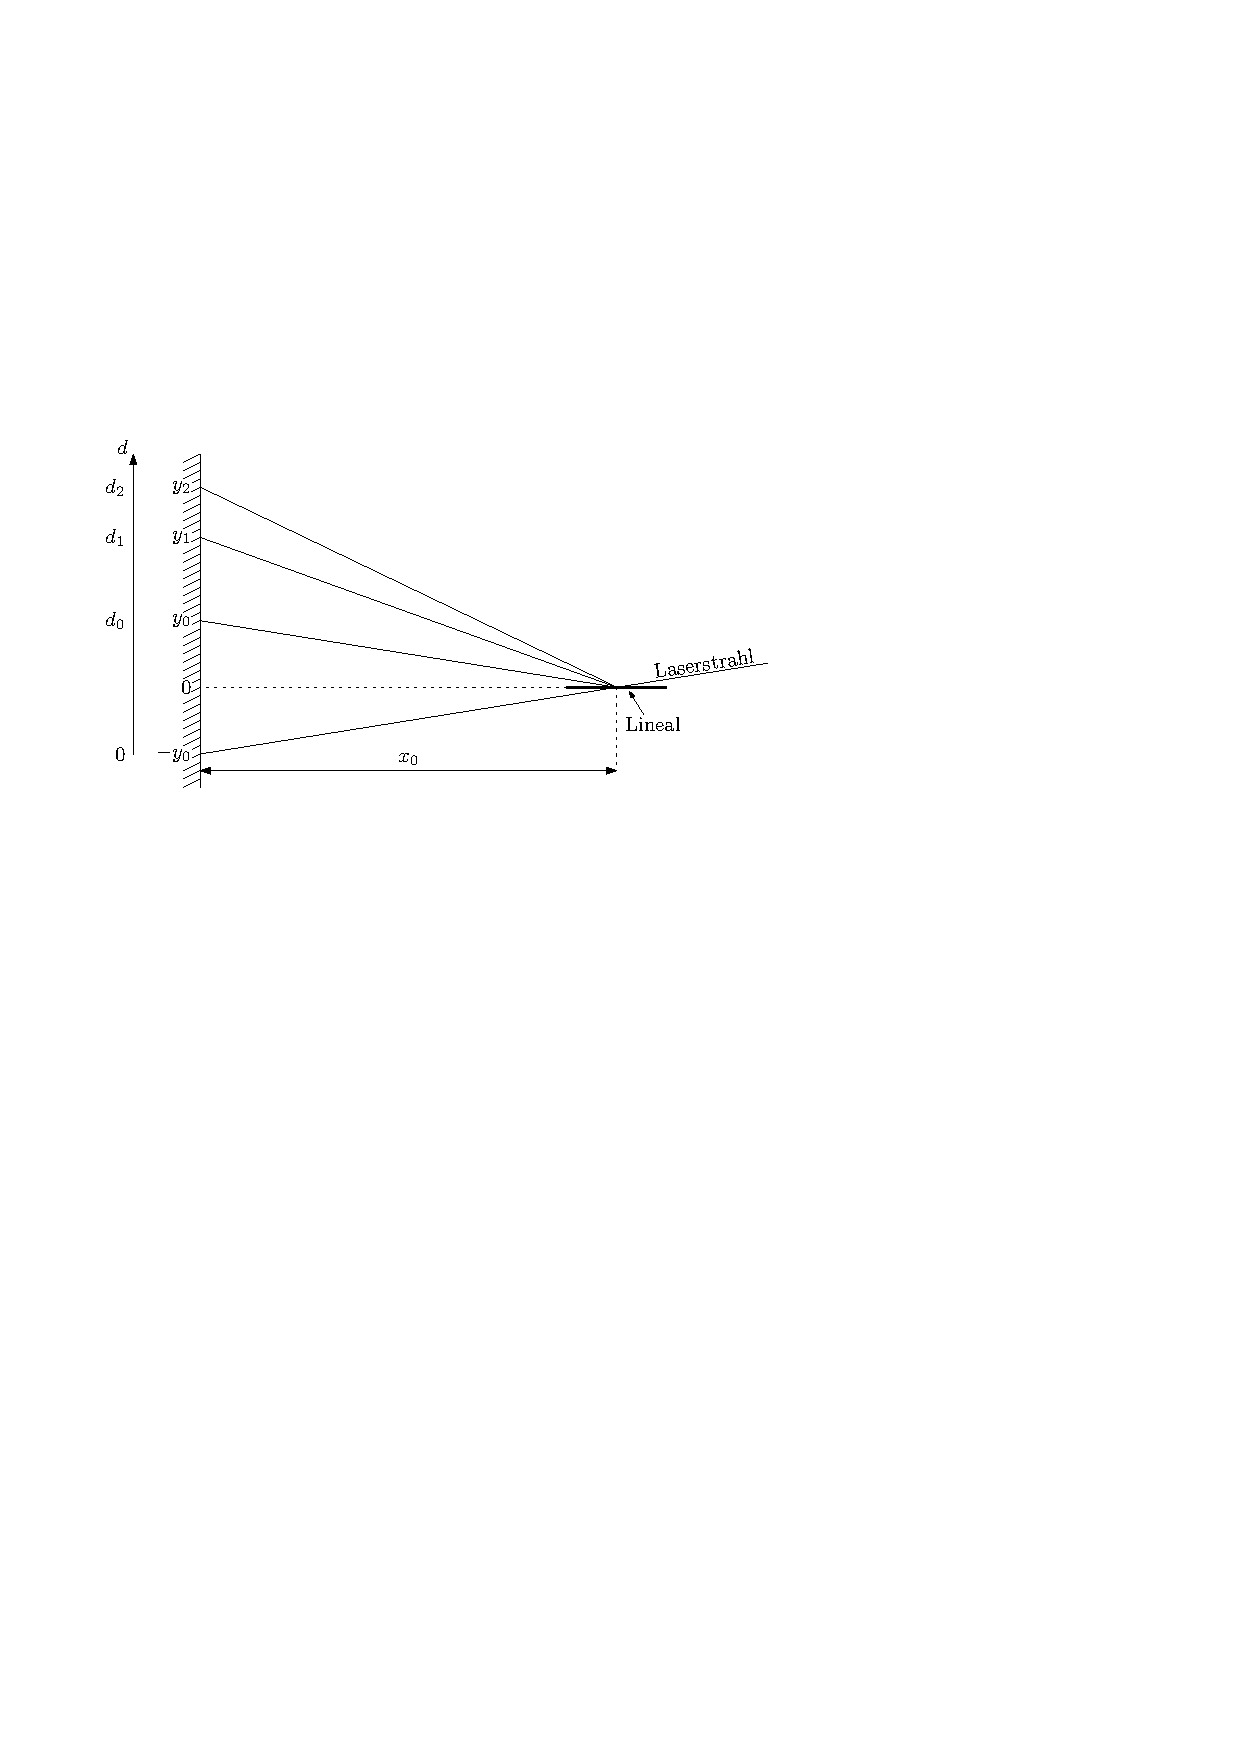
\includegraphics[width=0.9\textwidth]{./figures/wellenlaenge_lineal.pdf}
	\caption{Wellenlängenbestimmung nach Schawlow \cite{schawlow} und die im Versuch gemessenen Längen $d$}
	\label{fig:schawlow}
\end{figure}
Zur Bestimmung der Wellenlänge des Helium-Neon Lasers nach Schawlow \cite{schawlow} wird ein Stahlmaßstab mit eingravierter Skaleneinteilung als Reflexionsgitter verwendet.
Dazu wird der Laserstrahl in flachem Winkel auf die Millimeter-Skala des Maßstabes geleitet, sodass ein scharfes Interferenzmuster auf dem Whiteboard in einer Entfernung (von der Mitte der beleuchteten Stelle am Lineal) von $x_0 = \SI{252 +- 2}{\centi\metre}$ entsteht.
Anschließend werden die Maxima des Musters markiert, wobei darauf geachtet werden muss, dass bei der nullten Beugungsordnung begonnen wird, um negative Beugungsordnungen zu vermeiden.
Die nullte Beugungsordnung kann daran erkannt werden, dass sie maximale Intensität aufweist.
Nachdem ausreichend viele Ordnungen markiert wurden, wird das Lineal aus dem Strahlengang entfernt und der Auftreffpunkt des Laserstrahls auf dem Whiteboard markiert.
Schließlich wird mit einem Maßband die Position $d$ aller Beugungsmaxima relativ zum Auftreffpunkt des Lasers ohne Lineal gemessen (vergleiche dazu auch Abbildung \ref{fig:schawlow}).
Die Schärfe des Interferenzmusters ließ es dabei zu, die Längen $d$ mit einem abgeschätzten Fehler von $\Delta d = \SI{0.4}{\centi\metre}$ zu bestimmen, wobei die Hauptfehlerquelle in der Bestimmung des Intensitätsmaximums liegt und nicht in der Längenmessung mit dem Maßband.

\subsubsection{Auswertung}
In \cite{schawlow} wird gezeigt, dass für die Gittergleichung in Kleinwinkelnäherung ($\frac{y_n}{x_0} \ll 1$) gegeben ist:
\begin{align}
	n \lambda = \frac{1}{2} g \left( \frac{y_n^2 - y_0^2}{x_0^2} \right) \text{,}
	\label{eq:gittergleichung_schawlow}
\end{align}
wobei $g$ die Gitterkonstante ist und ansonsten die Notation aus Abbildung \ref{fig:schawlow} verwendet wird.
Um aus den gemessenen Werten $d_n$ die Wellenlänge zu bestimmen, muss zunächst die Position $y_0$ des reflektierten Strahls auf dem Schirm berechnet werden, welche gemäß Abbildung \ref{fig:schawlow} gegeben ist durch:
\begin{align}
	y_0 = \frac{d_0}{2} \text{,}
\end{align}
sodass mit dem gemessenen Wert $d_0 = \SI{19.7 +- 0.4}{\centi\metre}$ folgt:
\begin{align}
	y_0 = \SI{9.85 +- 0.20}{\centi\metre} \text{.}
\end{align}
So kann die Position $y_n$ des $n$-ten Interferenzmaximums berechnet werden durch:
\begin{align}
	y_n &= d_n - y_0 \\
	\Delta y_n &= \sqrt{\Delta d_n^2 + \Delta y_0^2}
\end{align}
und anschließend mit der genäherten Gittergleichung \ref{eq:gittergleichung_schawlow} die Wellenlänge des Lasers für die einzelnen Maxima berechnet werden, wobei für die Gitterkonstante $g = \SI{1}{\milli\metre}$ gilt, da die Beugung an der Millimeter-Skala des Maßstabes stattfindet. 
Der Fehler der berechneten Wellenlänge $\Delta \lambda$ ist gegeben durch Gauß'sche Fehlerfortpflanzung unter der Vernachlässigung des Fehlers in der Gitterkonstanten $g$:
\begin{align}
	\Delta \lambda = \frac{g}{2 n} \sqrt{\left( \frac{2 y_n}{x_0^2} \right)^2 \cdot \Delta y_n^2 + \left( \frac{2 y_0}{x_0^2} \right)^2 \cdot \Delta y_0^2 + \left(\frac{2\left(y_n^2 - y_0^2 \right)}{x_0^3}\right)^2 \cdot \Delta x_0^2} \text{.}
\end{align}
Die gemessenen Abstände $d$ sowie die berechneten Werte wurden in Tabelle \ref{tab:wellenlaengen_berechnung} aufgetragen.
\begin{table}[h]
	\centering
	\begin{tabular}{SSSSSSS}
\toprule
{$n$} & {$d_n$ / \si{\centi\metre}} & {$\Delta d_n$ / \si{\centi\metre}} & {$y_n$ / \si{\centi\metre}} & {$\Delta y_n$ / \si{\centi\metre}} & {$\lambda$ / \si{\nano\metre}} & {$\Delta \lambda$ / \si{\nano\metre}} \\
\midrule
1  & 23.2 & 0.2 & 13.35 & 0.23 & 639 & 51 \\
2  & 26.0 & 0.2 & 16.15 & 0.23 & 645 & 32 \\
3  & 28.1 & 0.2 & 18.25 & 0.23 & 619 & 25 \\
4  & 30.2 & 0.2 & 20.35 & 0.23 & 624 & 21 \\
5  & 32.0 & 0.2 & 22.15 & 0.23 & 620 & 19 \\
6  & 34.0 & 0.2 & 24.15 & 0.23 & 638 & 18 \\
7  & 35.4 & 0.2 & 25.55 & 0.23 & 625 & 17 \\
8  & 37.1 & 0.2 & 27.25 & 0.23 & 635 & 16 \\
9  & 38.5 & 0.2 & 28.65 & 0.23 & 633 & 16 \\
10 & 39.7 & 0.2 & 29.85 & 0.23 & 625 & 15 \\
11 & 41.3 & 0.2 & 31.45 & 0.23 & 639 & 15 \\
12 & 42.4 & 0.2 & 32.55 & 0.23 & 632 & 14 \\
13 & 43.5 & 0.2 & 33.65 & 0.23 & 627 & 14 \\
14 & 44.8 & 0.2 & 34.95 & 0.23 & 632 & 14 \\
15 & 46.0 & 0.2 & 36.15 & 0.23 & 635 & 14 \\
16 & 47.1 & 0.2 & 37.25 & 0.23 & 635 & 14 \\
17 & 47.9 & 0.2 & 38.05 & 0.23 & 626 & 13 \\
18 & 49.2 & 0.2 & 39.35 & 0.23 & 635 & 13 \\
19 & 50.4 & 0.2 & 40.55 & 0.23 & 641 & 13 \\
\bottomrule
\end{tabular}
	\caption{Messdaten und Berechnung zur Wellenlängenbestimmung}
	\label{tab:wellenlaengen_berechnung}
\end{table}
Um aus den berechneten Wellenlängen für die einzelnen Maxima eine Wellenlänge zu bestimmen, wird der varianzgewichtete Mittelwert:
\begin{align}
	\bar{\lambda} = \frac{\sum_i \frac{\lambda_i}{\Delta \lambda_i^2}}{\sum_i \frac{1}{\Delta \lambda_i^2}}
\end{align}
verwendet, wobei dessen Fehler gegeben ist durch:
\begin{align}
\Delta \bar{\lambda} = \frac{1}{\sqrt{\sum_i \frac{1}{\Delta \lambda_i^2}}} \text{.}
\end{align}
Mit den Werten aus Tabelle \ref{tab:wellenlaengen_berechnung} folgt für die varianzgewichtete mittlere Wellenlänge:
\begin{align}
	\bar{\lambda} = \SI{632.3 +- 5.6}{\nano\metre} \text{.}
\end{align}
Der Vergleich mit dem Literaturwert \cite{NISTSpectra} für den ($\mathrm{5s} \rightarrow \mathrm{3p}$)-Übergang von Neon:
\begin{align}
	\lambda = \SI{632.81646}{\nano\metre}
	\label{eq:HeNe_wellenlaenge}
\end{align}
liefert eine gute Übereinstimmung innerhalb des statistischen Fehlers.

\subsubsection{Vergleich mit der exakten Rechnung}
Im Folgenden soll der Einfluss der Näherung bei der Berechnung der Wellenlänge untersucht werden.
Dazu betrachtet man die Gittergleichung mit dem Einfallswinkel $\alpha$ und den Ausfallswinkel der $n$-ten Interferenzordnung $\beta_n$, welche jeweils zur Gitterebene gemessen werden (vergleiche Abbildung \ref{fig:schawlow}):
\begin{align}
	n \lambda = g \left( \cos(\alpha) - \cos(\beta_n) \right) \text{.}
	\label{eq:wellenlaenge_exakt}
\end{align}
Wegen $\alpha = \beta_0$ kann der Kosinus ausgedrückt werden als (Satz des Pythagoras):
\begin{align}
	\cos(\alpha) &= \frac{x_0}{\sqrt{x_0^2 + y_0^2}} \\
	\cos(\beta_n) &= \frac{x_0}{\sqrt{x_0^2 + y_n^2}} \text{,}
\end{align}
womit die relative Abweichung der Näherung von der exakten Rechnung aus den Gleichungen \ref{eq:gittergleichung_schawlow} und \ref{eq:wellenlaenge_exakt} folgt:
\begin{align}
	\frac{\Delta \lambda}{\lambda} = \frac{\lambda_\mathrm{KWN} - \lambda}{\lambda} = \frac{1}{2} \frac{\frac{y_n^2 - y_0^2}{x_0^2}}{ \frac{x_0}{\sqrt{x_0^2 + y_0^2}} - \frac{x_0}{\sqrt{x_0^2 + y_n^2}} } - 1
\end{align}
Diese Funktion ist in Abhängigkeit von $y_n$ in Abbildung \ref{fig:abweichung_wellenlaenge} aufgetragen, wobei für $y_0$ und $x_0$ die im Versuch gemessenen Werte verwendet werden.
\begin{figure}[h]
	\centering
	% GNUPLOT: LaTeX picture with Postscript
\begingroup
  \makeatletter
  \providecommand\color[2][]{%
    \GenericError{(gnuplot) \space\space\space\@spaces}{%
      Package color not loaded in conjunction with
      terminal option `colourtext'%
    }{See the gnuplot documentation for explanation.%
    }{Either use 'blacktext' in gnuplot or load the package
      color.sty in LaTeX.}%
    \renewcommand\color[2][]{}%
  }%
  \providecommand\includegraphics[2][]{%
    \GenericError{(gnuplot) \space\space\space\@spaces}{%
      Package graphicx or graphics not loaded%
    }{See the gnuplot documentation for explanation.%
    }{The gnuplot epslatex terminal needs graphicx.sty or graphics.sty.}%
    \renewcommand\includegraphics[2][]{}%
  }%
  \providecommand\rotatebox[2]{#2}%
  \@ifundefined{ifGPcolor}{%
    \newif\ifGPcolor
    \GPcolortrue
  }{}%
  \@ifundefined{ifGPblacktext}{%
    \newif\ifGPblacktext
    \GPblacktexttrue
  }{}%
  % define a \g@addto@macro without @ in the name:
  \let\gplgaddtomacro\g@addto@macro
  % define empty templates for all commands taking text:
  \gdef\gplbacktext{}%
  \gdef\gplfronttext{}%
  \makeatother
  \ifGPblacktext
    % no textcolor at all
    \def\colorrgb#1{}%
    \def\colorgray#1{}%
  \else
    % gray or color?
    \ifGPcolor
      \def\colorrgb#1{\color[rgb]{#1}}%
      \def\colorgray#1{\color[gray]{#1}}%
      \expandafter\def\csname LTw\endcsname{\color{white}}%
      \expandafter\def\csname LTb\endcsname{\color{black}}%
      \expandafter\def\csname LTa\endcsname{\color{black}}%
      \expandafter\def\csname LT0\endcsname{\color[rgb]{1,0,0}}%
      \expandafter\def\csname LT1\endcsname{\color[rgb]{0,1,0}}%
      \expandafter\def\csname LT2\endcsname{\color[rgb]{0,0,1}}%
      \expandafter\def\csname LT3\endcsname{\color[rgb]{1,0,1}}%
      \expandafter\def\csname LT4\endcsname{\color[rgb]{0,1,1}}%
      \expandafter\def\csname LT5\endcsname{\color[rgb]{1,1,0}}%
      \expandafter\def\csname LT6\endcsname{\color[rgb]{0,0,0}}%
      \expandafter\def\csname LT7\endcsname{\color[rgb]{1,0.3,0}}%
      \expandafter\def\csname LT8\endcsname{\color[rgb]{0.5,0.5,0.5}}%
    \else
      % gray
      \def\colorrgb#1{\color{black}}%
      \def\colorgray#1{\color[gray]{#1}}%
      \expandafter\def\csname LTw\endcsname{\color{white}}%
      \expandafter\def\csname LTb\endcsname{\color{black}}%
      \expandafter\def\csname LTa\endcsname{\color{black}}%
      \expandafter\def\csname LT0\endcsname{\color{black}}%
      \expandafter\def\csname LT1\endcsname{\color{black}}%
      \expandafter\def\csname LT2\endcsname{\color{black}}%
      \expandafter\def\csname LT3\endcsname{\color{black}}%
      \expandafter\def\csname LT4\endcsname{\color{black}}%
      \expandafter\def\csname LT5\endcsname{\color{black}}%
      \expandafter\def\csname LT6\endcsname{\color{black}}%
      \expandafter\def\csname LT7\endcsname{\color{black}}%
      \expandafter\def\csname LT8\endcsname{\color{black}}%
    \fi
  \fi
  \setlength{\unitlength}{0.0500bp}%
  \begin{picture}(7200.00,5040.00)%
    \gplgaddtomacro\gplbacktext{%
      \csname LTb\endcsname%
      \put(814,704){\makebox(0,0)[r]{\strut{} 0}}%
      \csname LTb\endcsname%
      \put(814,1383){\makebox(0,0)[r]{\strut{} 2}}%
      \csname LTb\endcsname%
      \put(814,2061){\makebox(0,0)[r]{\strut{} 4}}%
      \csname LTb\endcsname%
      \put(814,2740){\makebox(0,0)[r]{\strut{} 6}}%
      \csname LTb\endcsname%
      \put(814,3418){\makebox(0,0)[r]{\strut{} 8}}%
      \csname LTb\endcsname%
      \put(814,4097){\makebox(0,0)[r]{\strut{} 10}}%
      \csname LTb\endcsname%
      \put(814,4775){\makebox(0,0)[r]{\strut{} 12}}%
      \csname LTb\endcsname%
      \put(946,484){\makebox(0,0){\strut{} 0}}%
      \csname LTb\endcsname%
      \put(2117,484){\makebox(0,0){\strut{} 20}}%
      \csname LTb\endcsname%
      \put(3289,484){\makebox(0,0){\strut{} 40}}%
      \csname LTb\endcsname%
      \put(4460,484){\makebox(0,0){\strut{} 60}}%
      \csname LTb\endcsname%
      \put(5632,484){\makebox(0,0){\strut{} 80}}%
      \csname LTb\endcsname%
      \put(6803,484){\makebox(0,0){\strut{} 100}}%
      \put(176,2739){\rotatebox{-270}{\makebox(0,0){\strut{}$\frac{\lambda}{\lambda} \, / \, \si{\percent}$}}}%
      \put(3874,154){\makebox(0,0){\strut{}$y_n \, / \, \si{\centi\metre}$}}%
      \put(3874,4665){\makebox(0,0){\strut{}}}%
    }%
    \gplgaddtomacro\gplfronttext{%
      \csname LTb\endcsname%
      \put(5816,877){\makebox(0,0)[r]{\strut{}relative Abweichung}}%
    }%
    \gplbacktext
    \put(0,0){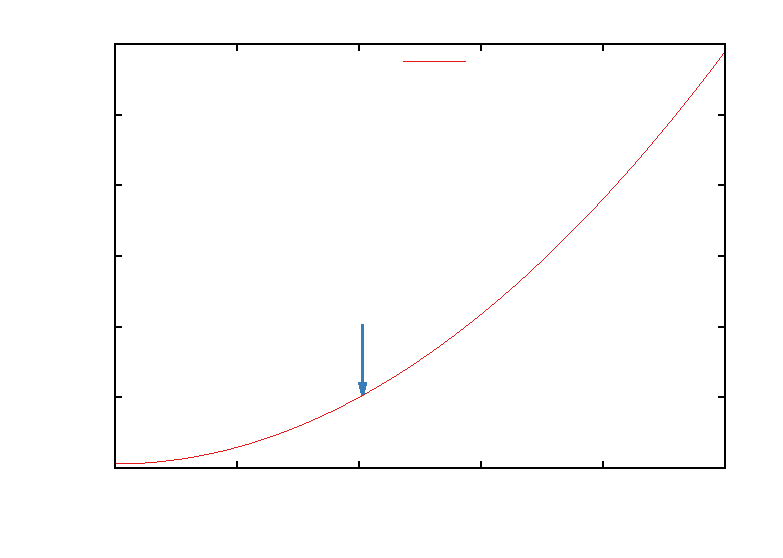
\includegraphics{./plots/abweichung_wellenlaenge}}%
    \gplfronttext
  \end{picture}%
\endgroup

	\caption{Relative Abweichung der Näherungsformel von der exakten Berechnung bei der im Versuch verwendeten Konfiguration: $y_0 = \SI{9.85}{\centi\metre}$, $x_0 = \SI{252}{\centi\metre}$. Der blaue Pfeil markiert die größte vermessene Interferenzordnung $n = 19$.}
	\label{fig:abweichung_wellenlaenge}
\end{figure}
Man sieht, dass die Abweichung für größere Ordnungen $n$ und damit größere Abstände $y_n$ rapide zunimmt, da $\frac{y_n}{x_0} \ll 1$ nicht mehr gegeben ist.
Demnach weist die größte vermessene Ordnung $n = \num{19}$ die größte relative Abweichung auf, welche wie man in Abbildung \ref{fig:abweichung_wellenlaenge} ablesen kann $\Delta \lambda / \lambda \approx \SI{2}{\percent}$ beträgt.
Dies entspricht schon einer Überschätzung der Wellenlänge von mehr als \SI{10}{\nano\metre} und liegt damit schon in der Größenordnung des statistischen Fehlers der Einzelmessungen.
Bemerkenswert ist, dass wir die Tendenz die Wellenlänge zu überschätzen in Messdaten nicht beobachtet werden kann, weshalb davon ausgegangen werden muss, dass ein systematischer Fehler diese kompensiert.
Eine mögliche Ursache kann sein, dass das Lineal einen kleinen Winkel zur Senkrechten auf der Wand aufwies und somit eine tendenzielle Unterschätzung der berechneten Wellenlänge zur Folge hat.

\subsection{Untersuchung der Polarisation des Lasers}
\label{ssec:polarisation}
Zur Untersuchung der Polarisation des hier verwendeten Experimentierlasers wird der Intensitätsverlauf an einer Photodiode in Abhängigkeit des Winkels eines davor stehenden Linearpolarisators betrachtet.
Dieser ist in der Lage, einfallendes Licht in eine vorgegebene Richtung linear zu polarisieren.
Für den Fall, dass das einfallende Licht bereits linear polarisiert ist (wie für den hier verwendeten Laser angenommen werden kann), gilt für die hinter dem Polarisator registrierte Intensität (Gesetz von Malus):
\begin{align}
I=I_0\cdot\cos^2\varphi
\end{align}

\subsubsection{Überprüfung des Gesetzes von Malus}
Der Winkel $\varphi$ am Polarisator wurde in Schritten von \SI{10}{\degree} gedreht und jeweils die Photospannung $U_\text{P}$ an der Photodiode in \si{\milli\volt} notiert.
In Tabelle \ref{tab:malus} sind die Messwerte bei einer Resonatorlänge von \SI{50}{\centi\metre} festgehalten worden.
Der Fehler $\Delta\varphi$ für den Winkel ergibt sich aus der Tatsache, dass der Polarisator in Schritten von \SI{2}{\degree} eingestellt werden konnte, der Fehler für die Photospannung wurde aufgrund der Schwankungen, die zu beobachten waren (es wurde mit der \emph{Measure}-Funktion des Oszilloskops gemessen), auf \SI{0.3}{\milli\volt} abgeschätzt.
Diese Messwerte werden im Anschluss mit \eqref{eq:umrechnung_watt} in Intensitäten umgerechnet, in ein Diagramm eingetragen und mit \texttt{Gnuplot} eine Kurve der Form
\begin{align}
f(x) = a\cdot\cos^2(x-b) + c
\end{align}
an die Daten angepasst.
Dabei beschreibt $a$ die Intensität $I_0$, der Parameter $b$ berücksichtigt eine eventuelle Abweichung, dass die Polarisatoreinstellung $\varphi=0$ nicht der Polarisationsrichtung des Lasers entspricht und $c$ beschreibt den auftretenden Untergrund der Spannungs- / Intensitätsmessung.
Als Ergebnis der Anpassung erhält man
\begin{align}
a&=\SI{2.24+-0.04}{\milli\watt}\\
b&=\SI{1.7+-0.6}{\degree}\\
c&=\SI{0.04+-0.03}{\milli\watt}
\end{align}
bei einem reduzierten $\chi^2$ von \num{25.4}.
\begin{figure}
	\centering
	\begin{tabular}{SSSS}
	\toprule
	{Drehwinkel $\varphi / \si{\degree}$} & {Fehler $\Delta\varphi / \si{\degree}$} & {Intensität $I / \si{\milli\volt}$} & {Fehler $\Delta I / \si{\milli\volt}$} \\
	\midrule
	0   & 1 & 39.50 & 0.3 \\
	10  & 1 & 40.00 & 0.3 \\
	20  & 1 & 38.00 & 0.3 \\
	30  & 1 & 33.80 & 0.3 \\
	40  & 1 & 27.90 & 0.3 \\
	50  & 1 & 20.20 & 0.3 \\
	60  & 1 & 13.40 & 0.3 \\
	70  & 1 & 6.45  & 0.3 \\
	80  & 1 & 2.62  & 0.3 \\
	90  & 1 & 0.60  & 0.3 \\
	100 & 1 & 1.10  & 0.3 \\
	110 & 1 & 3.50  & 0.3 \\
	120 & 1 & 8.60  & 0.3 \\
	130 & 1 & 14.70 & 0.3 \\
	140 & 1 & 21.20 & 0.3 \\
	150 & 1 & 27.70 & 0.3 \\
	160 & 1 & 33.40 & 0.3 \\
	170 & 1 & 37.00 & 0.3 \\
	180 & 1 & 38.50 & 0.3 \\
	190 & 1 & 37.50 & 0.3 \\
	200 & 1 & 34.70 & 0.3 \\
	210 & 1 & 29.60 & 0.3 \\
	220 & 1 & 22.90 & 0.3 \\
	230 & 1 & 16.30 & 0.3 \\
	240 & 1 & 9.50  & 0.3 \\
	250 & 1 & 4.10  & 0.3 \\
	260 & 1 & 1.30  & 0.3 \\
	270 & 1 & 0.30  & 0.3 \\
	280 & 1 & 2.00  & 0.3 \\
	290 & 1 & 5.60  & 0.3 \\
	300 & 1 & 10.90 & 0.3 \\
	310 & 1 & 17.60 & 0.3 \\
	320 & 1 & 24.40 & 0.3 \\
	330 & 1 & 30.50 & 0.3 \\
	340 & 1 & 35.60 & 0.3 \\
	350 & 1 & 38.70 & 0.3 \\
	360 & 1 & 39.50 & 0.3 \\
	\bottomrule
\end{tabular}
	\caption{Anpassung einer zu erwartenden Kurve an die Messwerte}
	\label{fig:malus}
\end{figure}
Man kann an der Anpassung gut erkennen, dass die Intensität wie erwartet dem Gesetz von Malus folgt.
Dies bestätigt auch die Annahme, dass der Laser durch die an der Entladungsröhre befestigten Brewster-Fenster mit linear polarisiertem Licht betrieben wird.
Die Abweichungen der Anpassung (das reduzierte $\chi^2$ von \num{25.4} bestätigt die schlechte Übereinstimmung) von den Messwerten lassen sich durch eine nicht ideale Justage erklären.
ERKLÄRUNG
Grund für die Annahme ist, dass das Maximum bei \SI{180}{\degree} nicht den zu erwartenden gleichen Wert annimmt, wie die Maxima bei \SI{0}{\degree} bzw. \SI{360}{\degree}.

\subsubsection{Polarisationsgrad des Lasers}
Nachfolgend soll der Polarisationsgrad des Lasers bestimmt werden.
Dieser ist gegeben durch:
\begin{align}
P=\frac{|I_{\parallel}-I_{\perp}|}{I_{\parallel}+I_{\perp}}
\end{align}
Der Fehler ergibt sich mit Gauß'scher Fehlerfortpflanzung zu:
\begin{align}
\Delta P=\sqrt{\left(1+\frac{I_{\perp}}{(I_{\parallel}+I_{\perp})^2}\right)^2\left(\Delta I_{\parallel}\right)^2 + \left(\frac{I_{\perp}}{(I_{\parallel}+I_{\perp})^2}-\frac{1}{I_{\parallel}+I_{\perp}}\right)^2\left(\Delta I_{\perp}\right)^2}
\end{align}
Hierbei wird angenommen, dass $I_\parallel$ die Intensität ist, bei der der Linearpolarisaor parallel zur Polarisationsrichtung des Lichts steht und so ein Transmissionsmaximum erreicht wird.
Für $I_\perp$ ist die Polarisationsrichtung des Lichts senkrecht zur Richtung des Polarisators, es liegt ein Transmisssionsminimum vor.
Aus der Anpassung (s.o.) kann die maximale Intensität als Summe der Anpassungsparameter $a$ und $c$ geschrieben werden, das Minimum ist gerade gleich $c$. 
Dann ergibt sich $P$ mit $I_\parallel=\SI{2.28+-0.05}{\milli\watt}$ und $I_\perp=\SI{0.04+-0.03}{\milli\watt}$ (die Fehler wurden mit Gauß'scher Fehlerfortpflanzung berechnet) zu:
\begin{align}
P=\num{0.97+-0.06}
\end{align}
Daran kann man sehen, dass das hier verwendete Laserlicht sehr stark (linear) polarisiert ist.

\subsection{Messung des Strahlprofils und des Stabilitätsgebiets des Lasers}
Im Folgenden soll das Strahlprofil im Resonator bei verschiedenen Resonatorlängen bestimmt werden.
Es werden dabei beispielhaft für eine Resonatorlänge Tabellen und Graphen in diesem Abschnitt aufgeführt.
Eine Zusammenstellung aller vermessenen Resonatorlängen findet sich in Anhang \ref{app:strahlprofil}.

\subsubsection{Messmethode}
Die Messung der Strahlprofils, beziehungsweise einer dazu proportionalen Größe (siehe Abschnitt \ref{sssec:spaltbreite_strahlradius}), erfolgt mithilfe eines Messschiebers, der in den Strahlengang gebracht wird.
Dabei wird die in \cite{anleitung} dargestellte Methode, bei der der Messschieber bei konstanter Spaltbreite longitudinal im Resonator verschoben wird, verwendet.
Konkret wird der Messschieber auf die konstante Breite $d$ eingestellt und an eine Position im Resonator gebracht, an der bei transversaler Verschiebung der Laser kurz aufblitzt.
Dann wird dessen Abstand $z$ vom ebenen Resonatorspiegel langsam vergrößert und beobachtet, wann der Strahl nichtmehr aufleuchtet, wenn der Messschieber gegen die Strahlachse bewegt wird.
Ist dieser Punkt erreicht, so wird der Abstand $z$ wieder verkleinert bis der Laser gerade noch anfängt zu arbeiten.
Dann kann der Abstand $z$ des Messschiebers vom ebenen Resonatorspiegel vermessen werden.
Dieser ist gleichzeitig der Abstand von der Strahltaille, da diese bei halbsymmetrischen Resonatoren auf dem ebenen Spiegel liegt (siehe auch Abschnitt (REF!)).

Bei dieser Methode treten Fehler in der Bestimmung der Position $z$ des Messschiebers und dessen Spaltbreite $d$ auf.
Der Fehler in der Position setzt sich zusammen aus dem Messfehler sowie einem zusätzlichen Beitrag aufgrund von nicht optimaler Ausrichtung (senkrecht zur optischen Achse) des Messschiebers.
Dazu kommt, dass die Position $z$ hinter dem Resonator nicht direkt mit der auf der optischen Bank angebrachten Skala vermessen werden konnte, weshalb für Messpunkte hinter dem Resonator ein größerer Fehler angenommen wurde, als für solche vor dem Resonator.
Der Fehler in der Spaltbreite $d$ ist im Wesentlichen nicht durch die Messung mit der Messschieber gegeben, sondern liegt darin, dass die (der unterschied $d = \pm \SI{0.01}{\milli\metre}$ kaum erkennbar).
Daher wird der statistische Fehler der Spaltbreite auf $\Delta d = \SI{0.01}{\milli\metre}$ abgeschätzt.
\begin{table}[h]
	\centering
	\begin{tabular}{SSSS}
\toprule
{$z \, / \, \si{\milli\metre}$} & {$\Delta z \, / \, \si{\milli\metre}$} & {$d \, / \, \si{\milli\metre}$} & {$\Delta d \, / \, \si{\milli\metre}$} \\
\midrule
10  & 2 & 0.67 & 0.01 \\
27  & 2 & 0.68 & 0.01 \\
442 & 4 & 1.04 & 0.01 \\
492 & 4 & 1.10 & 0.01 \\
542 & 4 & 1.16 & 0.01 \\
581 & 4 & 1.21 & 0.01 \\
639 & 4 & 1.26 & 0.01 \\
674 & 4 & 1.31 & 0.01 \\
708 & 4 & 1.36 & 0.01 \\
744 & 4 & 1.38 & 0.01 \\
\bottomrule
\end{tabular}
	\caption{Messdaten zum Strahlprofil im Resonator der Länge $L = \SI{795 +- 4}{\milli\metre}$}
	\label{tab:ex_messdaten_strahlprofil}
\end{table}


\subsubsection{Zusammenhang zwischen Spaltbreite $d$ und Strahlradius $w$}
\label{sssec:spaltbreite_strahlradius}
Zunächst gilt es zu beachten, dass der Strahlradius $w$ keine scharfe Begrenzung der transversalen Intensitätsverteilung eines Gaußstrahls darstellt.
Wie in Abschnitt (REF) erklärt, ist das transversale Profil der $\mathrm{TM}_{00}$-Mode gegeben durch durch eine Gaußfunktion, anhand derer der Strahlradius definiert ist als der Abstand von der Strahlachse, bei dem die Intensität auf $1/\mathrm{e}^2$ abgefallen ist.
Durch Begrenzung der der transversalen Strahlbreite auf die Spaltbreite des Messschiebers $d$, kommt es zu zusätlichen Verlusten aufgrund von Reflexion und Absorptions an den Backen des Messschiebers.
Diese Verluste führen zu einer Änderung der Schwellenbedingung für Laseroperation, was bei dieser Messmethode ausgenutzt wird, um eine zum Strahlradius $w$ proportionale Größe $d$ zu messen.
Da der Laser durch die Verschiebung des Messschiebers entlang der Strahlachse, stehts an der Schwelle operiert, ist die Strahlleistung im Spalt $P_\mathrm{Spalt}$ konstant bezüglich der verschiedener Messpositionen $z$.
Im Folgenden soll gezeigt werden, dass dann in der Tat gilt:
\begin{align}
	d = \alpha \cdot w(z) \text{,}
\end{align}
wobei $\alpha$ unabhängig vom Abstand $z$ von der Strahltaille ist.
Dazu betrachtet man die Leistung des Strahls auf der Fläche des durch den Messschiebers gebildeten Spaltes mit der Breite $d$:
\begin{align}
	P_\mathrm{Spalt} &= I_0 \left( \frac{w_0}{w(z)} \right)^2 \int_{A_\mathrm{Spalt}} \exp\left( -\frac{2 r^2}{w^2(z)} \right) \mathrm{d}A
\end{align}
mit $A_\mathrm{Spalt} = \left\{(x,y) \in \mathbb{R}^2 \middle| |x| < \frac{d}{2} \right\}$ und $r^2 = x^2 + y^2$.
Ausführen der Integration liefert die (konstante) Spaltleistung:
\begin{align}
	P_\mathrm{Spalt} &= \frac{1}{2} \pi I_0 w_0^2 \,\erf\left( \frac{d}{\sqrt{2} w(z)} \right)
\end{align}
Mit dem Ansatz $d(z) = \alpha(z) \cdot w(z)$ folgt:
\begin{align}
	\alpha(z) = \sqrt{2} \, \erf^{-1}\left( \frac{2}{\pi} \cdot \frac{P_\mathrm{Spalt}}{I_0 w_0^2}\right) = \mathrm{konst.}
\end{align}
Der Proportionalitätsfaktor $\alpha$ ist somit tatsächlich unabhängig von der Position des Messschiebers.

\subsubsection{Experimentelle Bestimmung des Strahlprofils}
Mit den Überlegungen aus dem vorigen Abschnitt wählen wir als Anpassungshypothese:
\begin{align}
	 r(z) = \frac{d(z)}{2} = \alpha \cdot w_\mathrm{exp.}(z) \text{,}
\end{align}
wobei das Profil $w_\mathrm{exp.}(z)$, unabhängig von der Rayleigh-Länge $z_0$, durch die Strahltaille $w_0$ ausgedrückt wird:
\begin{align}
	w_\mathrm{exp.}(z) = w_0 \sqrt{1 + \left( \frac{\lambda}{\pi} \right)^2 \left( \frac{z}{w_0^2}\right)^2}
\end{align}
(Folgerung aus Gleichungen \ref{eq:gauss_axialprofil} und \ref{eq:rayleigh_laenge}).
Das Halbieren\footnote{Auch der Fehler $\Delta r$ halbiert sich dementsprechend: $\Delta r = \Delta d / 2$} der Spaltbreite ist dabei optional und wurde durchgeführt um eine zum Strahlradius $w$ ähnlichere Größe zu erhalten.

Somit kann die Anpassung an die Messpunkte durch die \emph{Methode der kleinsten Quadrate} erfolgen.
Dabei werden die Proportionalitätskonstante $\alpha$ und die Strahltaille $w_0$ als Anpassungsparameter gewählt.
Die Messdaten, Anpassung, experimentelles und theoretisches Strahlprofil wurden in Abbildung \ref{fig:ex_strahlradius} aufgetragen.
Dabei ist der theoretische Strahlradius durch die aus der Resonatorgeometrie folgenden Strahltaille (Gleichung \ref{eq:strahltaille_halbsym}) gegeben.
Für die Wellenlänge des HeNe-Lasers wurde der Wert aus Gleichung \ref{eq:HeNe_wellenlaenge} verwendet.
Die resultierenden Anpassungsparameter für alle Resonatorlängen wurden in Tabelle \ref{tab:strahlradius_fitergebnis} aufgetragen.
\begin{table}[h]
	\centering
	\begin{tabular}{SSSSSSS}
\toprule
{$L \, / \, \si{\milli\metre}$} & {$\Delta L \, / \, \si{\milli\metre}$} & {$w_0 \, / \, \si{\milli\metre}$} & {$\Delta w_0 \, / \, \si{\milli\metre}$} & {$\alpha$} & {$\Delta \alpha$} & {$\chi_\mathrm{red.}^2$}\\
\midrule
500 & 4 & 0.3239 & 0.0029 & 1.149 & 0.005 & 0.52 \\
690 & 4 & 0.3093 & 0.0039 & 1.223 & 0.006 & 3.54 \\
795 & 4 & 0.2888 & 0.0052 & 1.195 & 0.010 & 6.23 \\
892 & 4 & 0.2557 & 0.0043 & 1.206 & 0.012 & 7.46 \\
\bottomrule
\end{tabular}
	\caption{Ergebnisse der Anpassung des Strahlprofils an die aufgenommenen Daten}
	\label{tab:strahlradius_fitergebnis}
\end{table}
\begin{figure}[h]
	\centering
	% GNUPLOT: LaTeX picture with Postscript
\begingroup
  \makeatletter
  \providecommand\color[2][]{%
    \GenericError{(gnuplot) \space\space\space\@spaces}{%
      Package color not loaded in conjunction with
      terminal option `colourtext'%
    }{See the gnuplot documentation for explanation.%
    }{Either use 'blacktext' in gnuplot or load the package
      color.sty in LaTeX.}%
    \renewcommand\color[2][]{}%
  }%
  \providecommand\includegraphics[2][]{%
    \GenericError{(gnuplot) \space\space\space\@spaces}{%
      Package graphicx or graphics not loaded%
    }{See the gnuplot documentation for explanation.%
    }{The gnuplot epslatex terminal needs graphicx.sty or graphics.sty.}%
    \renewcommand\includegraphics[2][]{}%
  }%
  \providecommand\rotatebox[2]{#2}%
  \@ifundefined{ifGPcolor}{%
    \newif\ifGPcolor
    \GPcolortrue
  }{}%
  \@ifundefined{ifGPblacktext}{%
    \newif\ifGPblacktext
    \GPblacktexttrue
  }{}%
  % define a \g@addto@macro without @ in the name:
  \let\gplgaddtomacro\g@addto@macro
  % define empty templates for all commands taking text:
  \gdef\gplbacktext{}%
  \gdef\gplfronttext{}%
  \makeatother
  \ifGPblacktext
    % no textcolor at all
    \def\colorrgb#1{}%
    \def\colorgray#1{}%
  \else
    % gray or color?
    \ifGPcolor
      \def\colorrgb#1{\color[rgb]{#1}}%
      \def\colorgray#1{\color[gray]{#1}}%
      \expandafter\def\csname LTw\endcsname{\color{white}}%
      \expandafter\def\csname LTb\endcsname{\color{black}}%
      \expandafter\def\csname LTa\endcsname{\color{black}}%
      \expandafter\def\csname LT0\endcsname{\color[rgb]{1,0,0}}%
      \expandafter\def\csname LT1\endcsname{\color[rgb]{0,1,0}}%
      \expandafter\def\csname LT2\endcsname{\color[rgb]{0,0,1}}%
      \expandafter\def\csname LT3\endcsname{\color[rgb]{1,0,1}}%
      \expandafter\def\csname LT4\endcsname{\color[rgb]{0,1,1}}%
      \expandafter\def\csname LT5\endcsname{\color[rgb]{1,1,0}}%
      \expandafter\def\csname LT6\endcsname{\color[rgb]{0,0,0}}%
      \expandafter\def\csname LT7\endcsname{\color[rgb]{1,0.3,0}}%
      \expandafter\def\csname LT8\endcsname{\color[rgb]{0.5,0.5,0.5}}%
    \else
      % gray
      \def\colorrgb#1{\color{black}}%
      \def\colorgray#1{\color[gray]{#1}}%
      \expandafter\def\csname LTw\endcsname{\color{white}}%
      \expandafter\def\csname LTb\endcsname{\color{black}}%
      \expandafter\def\csname LTa\endcsname{\color{black}}%
      \expandafter\def\csname LT0\endcsname{\color{black}}%
      \expandafter\def\csname LT1\endcsname{\color{black}}%
      \expandafter\def\csname LT2\endcsname{\color{black}}%
      \expandafter\def\csname LT3\endcsname{\color{black}}%
      \expandafter\def\csname LT4\endcsname{\color{black}}%
      \expandafter\def\csname LT5\endcsname{\color{black}}%
      \expandafter\def\csname LT6\endcsname{\color{black}}%
      \expandafter\def\csname LT7\endcsname{\color{black}}%
      \expandafter\def\csname LT8\endcsname{\color{black}}%
    \fi
  \fi
  \setlength{\unitlength}{0.0500bp}%
  \begin{picture}(7200.00,5040.00)%
    \gplgaddtomacro\gplbacktext{%
      \csname LTb\endcsname%
      \put(1078,704){\makebox(0,0)[r]{\strut{} 0,25}}%
      \csname LTb\endcsname%
      \put(1078,1074){\makebox(0,0)[r]{\strut{} 0,3}}%
      \csname LTb\endcsname%
      \put(1078,1444){\makebox(0,0)[r]{\strut{} 0,35}}%
      \csname LTb\endcsname%
      \put(1078,1814){\makebox(0,0)[r]{\strut{} 0,4}}%
      \csname LTb\endcsname%
      \put(1078,2184){\makebox(0,0)[r]{\strut{} 0,45}}%
      \csname LTb\endcsname%
      \put(1078,2554){\makebox(0,0)[r]{\strut{} 0,5}}%
      \csname LTb\endcsname%
      \put(1078,2925){\makebox(0,0)[r]{\strut{} 0,55}}%
      \csname LTb\endcsname%
      \put(1078,3295){\makebox(0,0)[r]{\strut{} 0,6}}%
      \csname LTb\endcsname%
      \put(1078,3665){\makebox(0,0)[r]{\strut{} 0,65}}%
      \csname LTb\endcsname%
      \put(1078,4035){\makebox(0,0)[r]{\strut{} 0,7}}%
      \csname LTb\endcsname%
      \put(1078,4405){\makebox(0,0)[r]{\strut{} 0,75}}%
      \csname LTb\endcsname%
      \put(1078,4775){\makebox(0,0)[r]{\strut{} 0,8}}%
      \csname LTb\endcsname%
      \put(1210,484){\makebox(0,0){\strut{} 0}}%
      \csname LTb\endcsname%
      \put(1909,484){\makebox(0,0){\strut{} 100}}%
      \csname LTb\endcsname%
      \put(2608,484){\makebox(0,0){\strut{} 200}}%
      \csname LTb\endcsname%
      \put(3307,484){\makebox(0,0){\strut{} 300}}%
      \csname LTb\endcsname%
      \put(4007,484){\makebox(0,0){\strut{} 400}}%
      \csname LTb\endcsname%
      \put(4706,484){\makebox(0,0){\strut{} 500}}%
      \csname LTb\endcsname%
      \put(5405,484){\makebox(0,0){\strut{} 600}}%
      \csname LTb\endcsname%
      \put(6104,484){\makebox(0,0){\strut{} 700}}%
      \csname LTb\endcsname%
      \put(6803,484){\makebox(0,0){\strut{} 800}}%
      \put(176,2739){\rotatebox{-270}{\makebox(0,0){\strut{}Strahlradius $w \, / \, \si{\milli\metre}$}}}%
      \put(4006,154){\makebox(0,0){\strut{}Abstand von der Strahltaille $z \, / \, \si{\milli\metre}$}}%
      \put(4006,4665){\makebox(0,0){\strut{}}}%
    }%
    \gplgaddtomacro\gplfronttext{%
      \csname LTb\endcsname%
      \put(3058,4602){\makebox(0,0)[r]{\strut{}Messwerte}}%
      \csname LTb\endcsname%
      \put(3058,4382){\makebox(0,0)[r]{\strut{}$\alpha \cdot w_\mathrm{exp.}(z)$}}%
      \csname LTb\endcsname%
      \put(3058,4162){\makebox(0,0)[r]{\strut{}$w_\mathrm{exp.}(z)$}}%
      \csname LTb\endcsname%
      \put(3058,3942){\makebox(0,0)[r]{\strut{}$w_\mathrm{theo.}(z)$}}%
    }%
    \gplbacktext
    \put(0,0){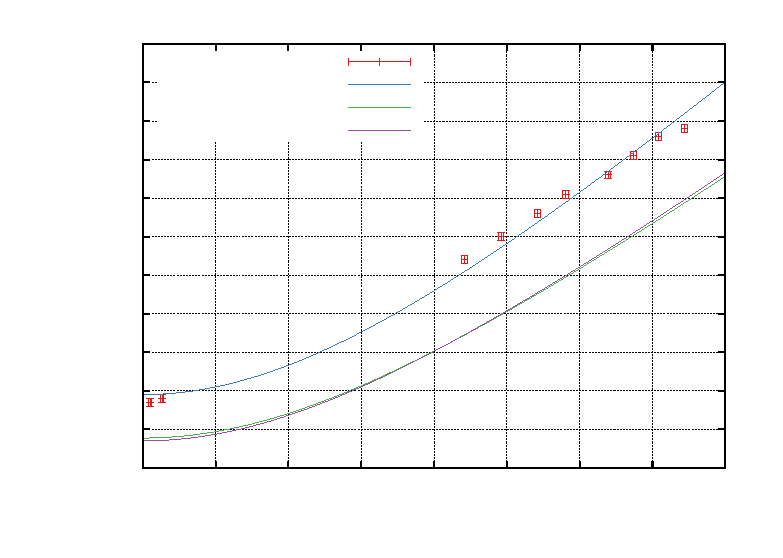
\includegraphics{./plots/strahlradien/strahlradius_80cm}}%
    \gplfronttext
  \end{picture}%
\endgroup

	\caption{Anpassung des Strahlprofils an die Messdaten für die Resonatorlänge $L = \SI{795 +- 4}{\milli\metre}$}
	\label{fig:ex_strahlradius}
\end{figure}

Bemerkenswert ist, dass man bei den letzten\footnote{bezogen auf den Abstand $z$ von der Strahltaille} Messpunkten im Strahlprofil ein systematisches Abknicken beobachten kann.
Die Ursache liegt vermutlich darin, dass an der Knickstelle das Aufblitzen des Lasers von der anderen Seite des Messschiebers beobachtet wurde, da der sphärische Resonatorspiegel den Blick auf den Messschieber beeinträchtigt hat.
Da der Reflexionsgrad beider Seiten des Messschiebers unterschiedlich ist, kommt es hier zu einem systematischen Fehler aufgrund der unterschiedlichen Helligkeiten des Reflexes an den Messbacken.

Zusammenfassend kann man sagen, dass des experimentell bestimmte Strahlprofil gut mit dem Theoretischen übereinstimmt.
Einzig für die Resonatorlänge $L = \SI{500}{\milli\metre}$ kommt es zu einer signifikanten Abweichung, da auf dem Messbereich nur wenige Messpunkte zur Verfügung standen.


\subsection{Aufbau der optischen Diode}

Die optische Diode wird in diesem Versuch durch eine Kombination von Linearpolarisator und $\lambda/4$-Platte erreicht.
Sie wird gemäß der Praktikumsanleitung aufgebaut und justiert.
Zur korrekten Einstellung der Diode wird der Polarisator nun so gedreht, dass das transmittierte Licht ein Maximum erreicht.
Hierfür findet man bei der Einstellung von \SI{254}{\degree} das Transmissionsminimum und verdreht den Polarisator um weitere \SI{90}{\degree} (dies folgt aus dem Gesetz von Malus, siehe Abschnitt \ref{ssec:polarisation}), so dass das Transmissionsmaximum bei einer Einstellung von \SI{344}{\degree} erreicht wird.\\
\\
Vor der optischen Diode kann bei der Resonatorlänge \SI{50}{\centi\metre} eine Intensität von \SI{66.2+-0.1}{\milli\volt} gemessen werden, hinter der Diode beträgt die Intensität \SI{47.2+-0.1}{\milli\volt}.
Die Leistungsverluste an der Diode (z.B. Reflexionen an der Vorderseite der $\lambda/4$-Platte) belaufen sich somit auf ca. \SI{1}{\milli\watt}.
Dabei wurde wie in \eqref{eq:umrechnung_watt} der Umrechnungsfaktor \num{17.5} zwischen der gemessenen Intensität in \si{\milli\volt} und \si{\milli\watt} verwendet.

\subsection{Optischer Spektrumanalysator}

\subsection{Präzise Messung des Modenabstandes mittels einer optischen Schwebung}
In diesem Teil soll der Modenabstand der longitudinalen Moden im Resonator durch eine optische Schwebung gemessen werden.
Dazu betrachtet man die Überlagerung des elektrischen Feldes zweier Axialmoden mit den Kreisfrequenzen $\omega_1$ und $\omega_2$ auf einer Photodiode.
Die Superposition der elektrischen Felder kann geschrieben werden als:
\begin{align}
	E(t) = E_1 \sin(\omega_1 t) + E_2 \sin(\omega_2 t)
	\label{eq:superposition_efeld}
\end{align}
Da die Photodiode die Intensität $I$ des auftreffenden Lichts misst und diese gegeben ist durch $I \propto E^2$, erhält man durch quadrieren von Gleichung \ref{eq:superposition_efeld} und Anwendung der trigonometrischen Additionstheoreme das resultierende Frequenzspektrum der Intensität, welche aus den Frequenzen $\omega_1 + \omega_2, |\omega_1 - \omega_2|$ sowie den zweiten Harmonischen $2\omega_1, 2\omega_2$ besteht.
Mit Ausnahme von dem Heterodynsignal mit der Frequenz $|\omega_1 - \omega_2|$, welche in der Größenordnung von einigen $\SI{100}{\mega\hertz}$ liegt, sind die restlichen auftretenden Frequenzen so groß ($\sim \si{\peta\hertz}$), dass diese aufgrund der endlichen Bandbreite der Photodiode ($\sim \si{\giga\hertz}$) nicht gemessen werden können.
Auch die Frequenz der optischen Schwebung ist so hoch, dass diese nicht direkt mit dem vorhandenen analogen Oszilloskop (Bandbreite $B = \SI{35}{\mega\hertz}$) gemessen werden kann.
Daher wird in einer zweiten Stufe das Signal der Schwebung mit dem eines Hochfrequenzgenerators der Frequenz $\nu_\mathrm{HF}$ gemischt.

\subsubsection{Mathematische Beschreibung der Funktionsweise eines Mischers}
Die Wirkung eines solchen \textbf{Mischers} auf zwei Eingangssignale $x(t) = \hat{x} \sin(\omega_1 t)$ und $y(t) = \hat{y} \sin(\omega_2 t)$ lässt sich auf zwei verschiedenen Weisen realisieren \cite{horowitz_hill}:
\begin{itemize}
	\item \textbf{multiplikative Mischung:} Durch Multiplikation der beiden Signale $x(t)$ und $y(t)$ führt die Anwendung der trigonometrischen Identität:
	\begin{align}
		\sin(\omega_1 t) \sin(\omega_2 t) = \frac{1}{2} \cos\left[ (\omega_1 - \omega_2) t \right] - \frac{1}{2} \cos\left[ (\omega_1 + \omega_2) t\right]
	\end{align}
	auf das resultierende Signal:
	\begin{align}
		(x\cdot y)(t) = \frac{\hat{x} \, \hat{y}}{2} \left\{ \cos\left[ (\omega_1 - \omega_2) t \right] - \cos\left[ (\omega_1 + \omega_2) t\right]\right\} \text{.}
	\end{align}
	Das resultierende Spektrum enthält sowohl die Summe als auch die Differenz der beiden Eingangsfrequenzen.
	\item \textbf{Mischung durch Anwendung einer nichtlinearen Operation auf die Summe der Signale:} Um die Differenzfrequenz $|\omega_1 - \omega_2|$ zu bestimmen, ist es nicht nötig das Produkt der beiden Eingänge zu bilden.
	Alternativ reicht es aus die Summe beider Signale zu bilden und eine nichtlineare Operation $f$ auf diese anzuwenden.
	Beschreibt man diese durch eine Potenzreihenentwicklung:
	\begin{align}
		f(x) = \sum_{n=0}^{\infty} a_n x^n
	\end{align}
	und wendet diese auf die Summe der Eingangssignale $(x+y)(t)$ an, so folgt für das Ausgangssignal:
	\begin{align}
		f(x+y)(t) = \sum_{n=0}^{\infty} a_n \left[ \hat{x} \sin(\omega_1 t) + \hat{y} \sin(\omega_2 t) \right]^n
	\end{align}
	Sofern mindestens einer der geraden Koeffizienten $a_n$ für $n = 2, 4, 6\dots$ nicht verschwindet, führt dies zum Auftreten eines Terms mit der Frequenz $|\omega_1 - \omega_2|$.
	Dies kann mit dem binomischen Lehrsatz sowie einigen trigonometrischen Identitäten gezeigt werden, dennoch soll hier darauf verzichtet werden.
	Der Spezialfall $f(x) = x^2$ ist bereits bei der Mischung der elektrischen Felder der verschiedenen Axialmoden in der Photodiode aufgetreten, da die gemessene Intensität quadratisch mit der Summe der Feldstärken $E_1$ und $E_2$ zusammenhängt.
	Demnach agiert bereits die Photodiode als Mischer für die elektrischen Feldstärken der verschiedenen Moden.
\end{itemize}

\subsubsection{Messung des Modenabstandes durch Mischung mit der Hochfrequenz}
Wie bereits erwähnt, wird das Signal der optischen Schwebung mit der Frequenz $\Delta \nu = |\omega_1 - \omega_2| / (2\pi)$ mit dem eines Hochfrequenzgenerators $\nu_\mathrm{HF}$ gemischt.
Dabei wird der \textbf{Leistungspegel} des Generators auf $L = \SI{+7}{\dBm}$ eingestellt. Um diese logarithmische Größe in Einheiten einer Leistung zu erhalten, betrachtet man die Definition des Leistungspegels $L$: 
\begin{align}
	L = 10 \cdot \log_{10}\left( \frac{P}{P_0}\right) \text{,}
\end{align}
wobei $P_0$ als Referenzgröße dient.
Für das Dezibel-Milliwatt (\si{dBm}) ist diese gegeben durch $P_0 = \SI{1}{\milli\watt}$, womit für die Leistung des Hochfrequenzgenerators folgt:
\begin{align}
	P = P_0 \cdot 10^{\frac{L}{10}} = \SI{1}{\milli\watt} \cdot 10^{\num{0.7}} \approx \SI{5}{\milli\watt}
\end{align}
Schließlich betrachtet man das Resultat der Mischung am Oszilloskop, welches die Differenzfrequenz $\nu = |\nu_\mathrm{HF} - \Delta \nu|$ aufweist.
Aufgrund der begrenzten Bandbreite des Oszilloskops ist es nötig, eine überschlagsmäßige Berechnung des Modenabstands $\Delta \nu$ durchzuführen, um einen Anhaltspunkt für die Frequenzeinstellung des Hochfrequenzgenerators zu erhalten.
Diese erfolgt über den theoretischen Axialmodenabstand:
\begin{align}
	\Delta \nu = \frac{c}{2 L} \text{,}
	\label{eq:modenabstand}
\end{align}
wobei $L$ die gemessene Resonatorlänge ist.
Fällt die Hochfrequenz $\nu_\mathrm{HF}$ und der Modenabstand $\Delta \nu$ innerhalb der Bandbreite des Oszilloskops zusammen, so kann ein sinusförmiges Signal gemessen werden.
(mehr Beschreibung zum Signal)
Anschließend wird die Hochfrequenz $\nu_\mathrm{HF}$ schrittweise verändert, sodass die Periode des Signals zunimmt.
Durch diese Methodik nähert man sich langsam der minimalen Signalfrequenz, wobei diese nicht beliebig genau bestimmt werden kann, da bei einer Annäherung in \SI{50}{\kilo\hertz}-Schritten das Signal in der Nähe des Minimums im Rauschen untergeht.
Ist dieser Punkt erreicht, wird die Frequenz des Signalgenerators notiert und dient als Approximation\footnote{Streng genommen müsste noch die Frequenz des Restsignals auf dem Oszilloskops vermessen werden. Da dieses aber im Rauschen nicht auszumachen ist und dessen Frequenz klein ist gegen den Modenabstand $\Delta \nu$, kann dieser Beitrag vernachlässigt werden.} des Modenabstandes $\Delta \nu$.
Aus der verwendeten Schrittbreite von \SI{50}{\kilo\hertz} folgt ein abgeschätzter Fehler für die Bestimmung des Frequenzminimums von $\Delta \nu_\mathrm{HF} = \SI{25}{\kilo\hertz}$ (halbe Schrittbreite).
Die gemessenen Modenabstände wurden in Tabelle \ref{tab:messdaten_optische_schwebung} aufgetragen.
\begin{table}[h]
	\centering
	\begin{tabular}{SSSS}
\toprule
  {$L \, / \, \si{\centi\metre}$} & {$\Delta L \, / \, \si{\centi\metre}$} & {$\nu_\mathrm{HF} \, / \, \si{\mega\hertz}$} & {$\Delta \nu_\mathrm{HF} \, / \, \si{\mega\hertz}$} \\
  \midrule
  50.0 & 0.4 & 299.360 & 0.025 \\ 
  69.0 & 0.4 & 216.150 & 0.025 \\
  79.5 & 0.4 & 187.450 & 0.025 \\
  89.2 & 0.4 & 168.650 & 0.025 \\
  \bottomrule
\end{tabular}
	\caption{Messwerte des longitudinalen Modenabstandes. Die eingestellte Hochfrequenz im Frequenzminimum approximiert den axialen Modenabstand $\nu_\mathrm{HF} \approx \Delta \nu$.}
	\label{tab:messdaten_optische_schwebung}
\end{table}

Diese Messwerte können im Hinblick auf den theoretischen Modenabstand in Gleichung \ref{eq:modenabstand} einen Wert für die Lichtgeschwindigkeit $c$ liefern.
Dazu wird die doppelte Resonatorlänge $2 L$ gegen die inverse Frequenz des Hochfrequenzgenerators im Frequenzminimum des gemischten Signals auf.
Der Graph sollte daher dem theoretischen Zusammenhang:
\begin{align}
	2 L = c \cdot \frac{1}{\nu_\mathrm{RF}}
\end{align}
folgen, wobei die Näherung $\Delta \nu \approx \nu_\mathrm{HF}$ verwendet wird.
Diese Form der Linearisierung wird gewählt, da bei einer Anpassung mit der \emph{Methode der kleinsten Quadrate} nur die Fehler in $y$-Richtung in die Gewichtung der Messpunkte eingehen.
Da der Fehler in der Frequenzbestimmung im Verhältnis zur Resonatorlängenbestimmung klein ist, wurde diese Form gewählt um eine sinnvolle Gewichtung bei der Geradenanpassung zu erzielen.
Mithilfe von \texttt{Gnuplot} wird eine Ursprungsgerade an die linearisierten Datenpunkte angepasst, wobei die Fehler gegeben sind durch:
\begin{align}
\Delta(2L) &= 2 \Delta L \\
\Delta \left( \frac{1}{\nu_\mathrm{HF}} \right) &= \frac{\Delta \nu_\mathrm{HF}}{\nu_\mathrm{HF}^2}
\end{align}
Die Linearisierung wurde in Abbildung \ref{fig:linearisierung_modenabstand} aufgetragen.
\begin{figure}[h]
	\centering
	% GNUPLOT: LaTeX picture with Postscript
\begingroup
  \makeatletter
  \providecommand\color[2][]{%
    \GenericError{(gnuplot) \space\space\space\@spaces}{%
      Package color not loaded in conjunction with
      terminal option `colourtext'%
    }{See the gnuplot documentation for explanation.%
    }{Either use 'blacktext' in gnuplot or load the package
      color.sty in LaTeX.}%
    \renewcommand\color[2][]{}%
  }%
  \providecommand\includegraphics[2][]{%
    \GenericError{(gnuplot) \space\space\space\@spaces}{%
      Package graphicx or graphics not loaded%
    }{See the gnuplot documentation for explanation.%
    }{The gnuplot epslatex terminal needs graphicx.sty or graphics.sty.}%
    \renewcommand\includegraphics[2][]{}%
  }%
  \providecommand\rotatebox[2]{#2}%
  \@ifundefined{ifGPcolor}{%
    \newif\ifGPcolor
    \GPcolortrue
  }{}%
  \@ifundefined{ifGPblacktext}{%
    \newif\ifGPblacktext
    \GPblacktexttrue
  }{}%
  % define a \g@addto@macro without @ in the name:
  \let\gplgaddtomacro\g@addto@macro
  % define empty templates for all commands taking text:
  \gdef\gplbacktext{}%
  \gdef\gplfronttext{}%
  \makeatother
  \ifGPblacktext
    % no textcolor at all
    \def\colorrgb#1{}%
    \def\colorgray#1{}%
  \else
    % gray or color?
    \ifGPcolor
      \def\colorrgb#1{\color[rgb]{#1}}%
      \def\colorgray#1{\color[gray]{#1}}%
      \expandafter\def\csname LTw\endcsname{\color{white}}%
      \expandafter\def\csname LTb\endcsname{\color{black}}%
      \expandafter\def\csname LTa\endcsname{\color{black}}%
      \expandafter\def\csname LT0\endcsname{\color[rgb]{1,0,0}}%
      \expandafter\def\csname LT1\endcsname{\color[rgb]{0,1,0}}%
      \expandafter\def\csname LT2\endcsname{\color[rgb]{0,0,1}}%
      \expandafter\def\csname LT3\endcsname{\color[rgb]{1,0,1}}%
      \expandafter\def\csname LT4\endcsname{\color[rgb]{0,1,1}}%
      \expandafter\def\csname LT5\endcsname{\color[rgb]{1,1,0}}%
      \expandafter\def\csname LT6\endcsname{\color[rgb]{0,0,0}}%
      \expandafter\def\csname LT7\endcsname{\color[rgb]{1,0.3,0}}%
      \expandafter\def\csname LT8\endcsname{\color[rgb]{0.5,0.5,0.5}}%
    \else
      % gray
      \def\colorrgb#1{\color{black}}%
      \def\colorgray#1{\color[gray]{#1}}%
      \expandafter\def\csname LTw\endcsname{\color{white}}%
      \expandafter\def\csname LTb\endcsname{\color{black}}%
      \expandafter\def\csname LTa\endcsname{\color{black}}%
      \expandafter\def\csname LT0\endcsname{\color{black}}%
      \expandafter\def\csname LT1\endcsname{\color{black}}%
      \expandafter\def\csname LT2\endcsname{\color{black}}%
      \expandafter\def\csname LT3\endcsname{\color{black}}%
      \expandafter\def\csname LT4\endcsname{\color{black}}%
      \expandafter\def\csname LT5\endcsname{\color{black}}%
      \expandafter\def\csname LT6\endcsname{\color{black}}%
      \expandafter\def\csname LT7\endcsname{\color{black}}%
      \expandafter\def\csname LT8\endcsname{\color{black}}%
    \fi
  \fi
  \setlength{\unitlength}{0.0500bp}%
  \begin{picture}(7200.00,5040.00)%
    \gplgaddtomacro\gplbacktext{%
      \csname LTb\endcsname%
      \put(946,704){\makebox(0,0)[r]{\strut{} 80}}%
      \csname LTb\endcsname%
      \put(946,1111){\makebox(0,0)[r]{\strut{} 90}}%
      \csname LTb\endcsname%
      \put(946,1518){\makebox(0,0)[r]{\strut{} 100}}%
      \csname LTb\endcsname%
      \put(946,1925){\makebox(0,0)[r]{\strut{} 110}}%
      \csname LTb\endcsname%
      \put(946,2332){\makebox(0,0)[r]{\strut{} 120}}%
      \csname LTb\endcsname%
      \put(946,2740){\makebox(0,0)[r]{\strut{} 130}}%
      \csname LTb\endcsname%
      \put(946,3147){\makebox(0,0)[r]{\strut{} 140}}%
      \csname LTb\endcsname%
      \put(946,3554){\makebox(0,0)[r]{\strut{} 150}}%
      \csname LTb\endcsname%
      \put(946,3961){\makebox(0,0)[r]{\strut{} 160}}%
      \csname LTb\endcsname%
      \put(946,4368){\makebox(0,0)[r]{\strut{} 170}}%
      \csname LTb\endcsname%
      \put(946,4775){\makebox(0,0)[r]{\strut{} 180}}%
      \csname LTb\endcsname%
      \put(1078,484){\makebox(0,0){\strut{} 3}}%
      \csname LTb\endcsname%
      \put(2032,484){\makebox(0,0){\strut{} 3,5}}%
      \csname LTb\endcsname%
      \put(2986,484){\makebox(0,0){\strut{} 4}}%
      \csname LTb\endcsname%
      \put(3941,484){\makebox(0,0){\strut{} 4,5}}%
      \csname LTb\endcsname%
      \put(4895,484){\makebox(0,0){\strut{} 5}}%
      \csname LTb\endcsname%
      \put(5849,484){\makebox(0,0){\strut{} 5,5}}%
      \csname LTb\endcsname%
      \put(6803,484){\makebox(0,0){\strut{} 6}}%
      \put(176,2739){\rotatebox{-270}{\makebox(0,0){\strut{}$2 L \, / \, \si{\centi\metre}$}}}%
      \put(3940,154){\makebox(0,0){\strut{}$\frac{1}{\nu_\mathrm{HF}} \, / \, \si{\nano\second}$}}%
      \put(3940,4665){\makebox(0,0){\strut{}}}%
    }%
    \gplgaddtomacro\gplfronttext{%
      \csname LTb\endcsname%
      \put(5816,1097){\makebox(0,0)[r]{\strut{}Datenpunkte}}%
      \csname LTb\endcsname%
      \put(5816,877){\makebox(0,0)[r]{\strut{}Anpassungsgerade}}%
    }%
    \gplbacktext
    \put(0,0){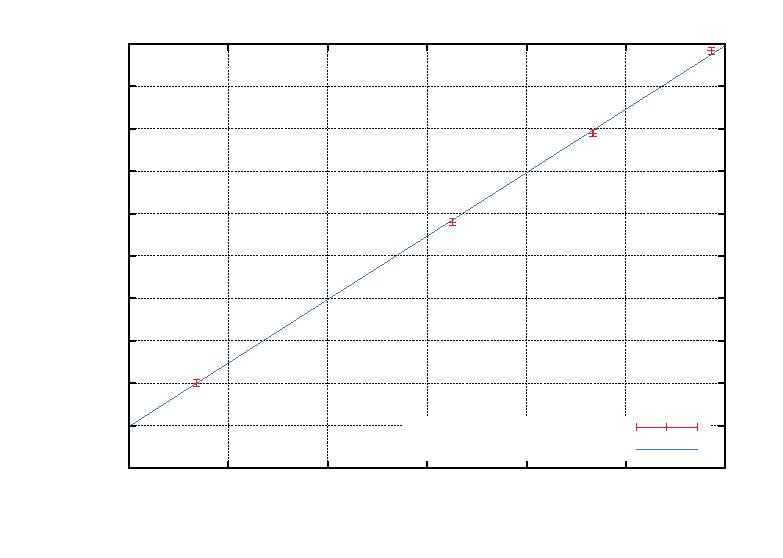
\includegraphics{./plots/linearisierung_modenabstand}}%
    \gplfronttext
  \end{picture}%
\endgroup

	\caption{Linearisierung des gemessenen Modenabstandes zur Bestimmung der Lichtgeschwindigkeit. Der Fehler der inversen Frequenz liegt innerhalb der Breite der Datenpunkte.}
	\label{fig:linearisierung_modenabstand}
\end{figure}
Die Güte der Anpassung ist gegeben durch das reduzierte Chi-Quadrat $\chi_\mathrm{red.}^2 = \num{0.8}$ und bestätigt das zugrundeliegende Modell.
Die Lichtgeschwindigkeit $c$ lässt sich sofort an der Steigung der angepassten Ursprungsgerade ablesen und ist gegeben durch:
\begin{align}
	c &= \SI{29.929 +- 0.073}{\centi\metre\per\nano\second} \nonumber\\
	&= \SI{2.9929 +- 0.0073 e8}{\metre\per\second}
\end{align}
Dieser Wert stimmt gut mit der Definition der Lichtgeschwindigkeit im Vakuum:
\begin{align}
	c_0 = \SI{299792458}{\metre\per\second}
\end{align}
überein.

\section{Fazit}
\clearpage
\section{Grafikstorage}
\begin{figure}[h]
\centering
\begin{tabular}{@{}lcccc|cc@{}}
\toprule
Nummer $i$   & $x_i$ / \si{\milli\second} & $\Delta(x_i)$ / \si{\milli\second} & $\Delta T$ / \si{\milli\second} & $\Delta(\Delta T)$ / \si{\milli\second} & $T_\text{konf.}$ / \si{\milli\second} & $\Delta T_\text{konf.}$ / \si{\milli\second} \\ \midrule
1            & 5.360  & 0.007   & \multirow{2}{*}{0.974} & \multirow{2}{*}{0.008}          & 4.474     & 0.011       \\
2            & 6.334  & 0,003   & \multirow{2}{*}{0,898} & \multirow{2}{*}{0,004}          & 4,271     & 0,004       \\
3            & 7,232  & 0,003   & \multirow{2}{*}{0,882} & \multirow{2}{*}{0,005}          & 4,145     & 0,005       \\
4            & 8,114  & 0,004   & \multirow{2}{*}{0,885} & \multirow{2}{*}{0,011}          & 4,051     & 0,005       \\
5            & 8,999  & 0,010   &                        &                & 3,947     & 0,023       \\
6            & 9,834  & 0,008   & \multirow{2}{*}{0,771} & \multirow{2}{*}{0,009}          &           &             \\
7            & 10,605 & 0,003   & \multirow{2}{*}{0,772} & \multirow{2}{*}{0,004}          &           &             \\
8            & 11,377 & 0,003   & \multirow{2}{*}{0,788} & \multirow{2}{*}{0,005}          &           &             \\
9            & 12,166 & 0,003   & \multirow{2}{*}{0,780} & \multirow{2}{*}{0,021}          &           &             \\
10           & 12,946 & 0,021   &                        &                &           &             \\
Mittelwert: &        &         & 0,840                  & 0,002          & 4,179     & 0,003       \\ \bottomrule
\end{tabular}
\caption{Resonatorlänge 50cm ALL0028}
\end{figure}
\begin{figure}[h]
\centering
% GNUPLOT: LaTeX picture with Postscript
\begingroup
  \makeatletter
  \providecommand\color[2][]{%
    \GenericError{(gnuplot) \space\space\space\@spaces}{%
      Package color not loaded in conjunction with
      terminal option `colourtext'%
    }{See the gnuplot documentation for explanation.%
    }{Either use 'blacktext' in gnuplot or load the package
      color.sty in LaTeX.}%
    \renewcommand\color[2][]{}%
  }%
  \providecommand\includegraphics[2][]{%
    \GenericError{(gnuplot) \space\space\space\@spaces}{%
      Package graphicx or graphics not loaded%
    }{See the gnuplot documentation for explanation.%
    }{The gnuplot epslatex terminal needs graphicx.sty or graphics.sty.}%
    \renewcommand\includegraphics[2][]{}%
  }%
  \providecommand\rotatebox[2]{#2}%
  \@ifundefined{ifGPcolor}{%
    \newif\ifGPcolor
    \GPcolortrue
  }{}%
  \@ifundefined{ifGPblacktext}{%
    \newif\ifGPblacktext
    \GPblacktexttrue
  }{}%
  % define a \g@addto@macro without @ in the name:
  \let\gplgaddtomacro\g@addto@macro
  % define empty templates for all commands taking text:
  \gdef\gplbacktext{}%
  \gdef\gplfronttext{}%
  \makeatother
  \ifGPblacktext
    % no textcolor at all
    \def\colorrgb#1{}%
    \def\colorgray#1{}%
  \else
    % gray or color?
    \ifGPcolor
      \def\colorrgb#1{\color[rgb]{#1}}%
      \def\colorgray#1{\color[gray]{#1}}%
      \expandafter\def\csname LTw\endcsname{\color{white}}%
      \expandafter\def\csname LTb\endcsname{\color{black}}%
      \expandafter\def\csname LTa\endcsname{\color{black}}%
      \expandafter\def\csname LT0\endcsname{\color[rgb]{1,0,0}}%
      \expandafter\def\csname LT1\endcsname{\color[rgb]{0,1,0}}%
      \expandafter\def\csname LT2\endcsname{\color[rgb]{0,0,1}}%
      \expandafter\def\csname LT3\endcsname{\color[rgb]{1,0,1}}%
      \expandafter\def\csname LT4\endcsname{\color[rgb]{0,1,1}}%
      \expandafter\def\csname LT5\endcsname{\color[rgb]{1,1,0}}%
      \expandafter\def\csname LT6\endcsname{\color[rgb]{0,0,0}}%
      \expandafter\def\csname LT7\endcsname{\color[rgb]{1,0.3,0}}%
      \expandafter\def\csname LT8\endcsname{\color[rgb]{0.5,0.5,0.5}}%
    \else
      % gray
      \def\colorrgb#1{\color{black}}%
      \def\colorgray#1{\color[gray]{#1}}%
      \expandafter\def\csname LTw\endcsname{\color{white}}%
      \expandafter\def\csname LTb\endcsname{\color{black}}%
      \expandafter\def\csname LTa\endcsname{\color{black}}%
      \expandafter\def\csname LT0\endcsname{\color{black}}%
      \expandafter\def\csname LT1\endcsname{\color{black}}%
      \expandafter\def\csname LT2\endcsname{\color{black}}%
      \expandafter\def\csname LT3\endcsname{\color{black}}%
      \expandafter\def\csname LT4\endcsname{\color{black}}%
      \expandafter\def\csname LT5\endcsname{\color{black}}%
      \expandafter\def\csname LT6\endcsname{\color{black}}%
      \expandafter\def\csname LT7\endcsname{\color{black}}%
      \expandafter\def\csname LT8\endcsname{\color{black}}%
    \fi
  \fi
  \setlength{\unitlength}{0.0500bp}%
  \begin{picture}(7200.00,5040.00)%
    \gplgaddtomacro\gplbacktext{%
      \csname LTb\endcsname%
      \put(946,704){\makebox(0,0)[r]{\strut{} 0}}%
      \csname LTb\endcsname%
      \put(946,1286){\makebox(0,0)[r]{\strut{} 50}}%
      \csname LTb\endcsname%
      \put(946,1867){\makebox(0,0)[r]{\strut{} 100}}%
      \csname LTb\endcsname%
      \put(946,2449){\makebox(0,0)[r]{\strut{} 150}}%
      \csname LTb\endcsname%
      \put(946,3030){\makebox(0,0)[r]{\strut{} 200}}%
      \csname LTb\endcsname%
      \put(946,3612){\makebox(0,0)[r]{\strut{} 250}}%
      \csname LTb\endcsname%
      \put(946,4193){\makebox(0,0)[r]{\strut{} 300}}%
      \csname LTb\endcsname%
      \put(946,4775){\makebox(0,0)[r]{\strut{} 350}}%
      \csname LTb\endcsname%
      \put(1078,484){\makebox(0,0){\strut{} 5}}%
      \csname LTb\endcsname%
      \put(1598,484){\makebox(0,0){\strut{} 6}}%
      \csname LTb\endcsname%
      \put(2119,484){\makebox(0,0){\strut{} 7}}%
      \csname LTb\endcsname%
      \put(2639,484){\makebox(0,0){\strut{} 8}}%
      \csname LTb\endcsname%
      \put(3160,484){\makebox(0,0){\strut{} 9}}%
      \csname LTb\endcsname%
      \put(3680,484){\makebox(0,0){\strut{} 10}}%
      \csname LTb\endcsname%
      \put(4201,484){\makebox(0,0){\strut{} 11}}%
      \csname LTb\endcsname%
      \put(4721,484){\makebox(0,0){\strut{} 12}}%
      \csname LTb\endcsname%
      \put(5242,484){\makebox(0,0){\strut{} 13}}%
      \csname LTb\endcsname%
      \put(5762,484){\makebox(0,0){\strut{} 14}}%
      \csname LTb\endcsname%
      \put(6283,484){\makebox(0,0){\strut{} 15}}%
      \csname LTb\endcsname%
      \put(6803,484){\makebox(0,0){\strut{} 16}}%
      \put(176,2739){\rotatebox{-270}{\makebox(0,0){\strut{}Photospannung $U_\text{PD} / \si{\milli\volt}$}}}%
      \put(3940,154){\makebox(0,0){\strut{}Zeitablenkung $T$ / \si{\milli\second}}}%
      \put(3940,4665){\makebox(0,0){\strut{}}}%
    }%
    \gplgaddtomacro\gplfronttext{%
      \csname LTb\endcsname%
      \put(5816,4602){\makebox(0,0)[r]{\strut{}Messwerte}}%
      \csname LTb\endcsname%
      \put(5816,4382){\makebox(0,0)[r]{\strut{}Anpassungskurve}}%
    }%
    \gplbacktext
    \put(0,0){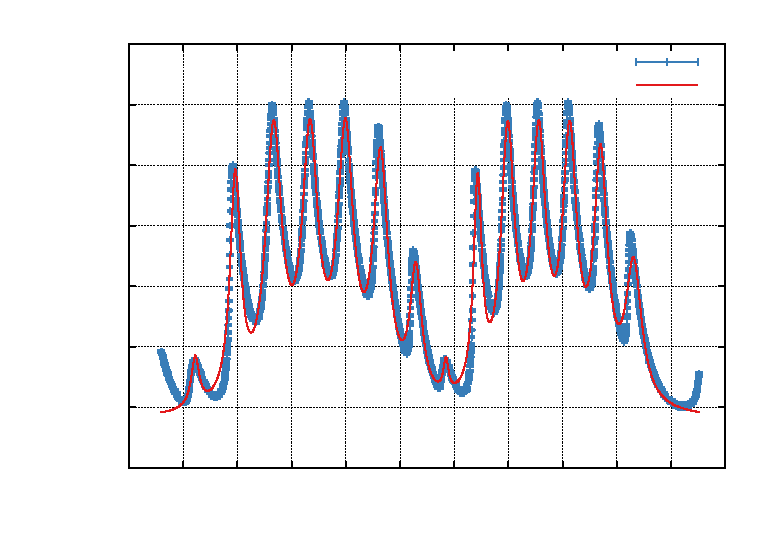
\includegraphics{./plots/modenabstand/ALL0026}}%
    \gplfronttext
  \end{picture}%
\endgroup

\caption{Resonatorlänge 70cm ALL0026}
\end{figure}
\begin{figure}[h]
\centering
\begin{tabular}{@{}lcccc|cc@{}}
\toprule
Nummer $i$   & $x_i$ / \si{\milli\second} & $\Delta(x_i)$ / \si{\milli\second} & $\Delta T$ / \si{\milli\second} & $\Delta(\Delta T)$ / \si{\milli\second} & $T_\text{konf.}$ / \si{\milli\second} & $\Delta T_\text{konf.}$ / \si{\milli\second} \\ \midrule
1  & 4,754  & 0,006 & \multirow{2}{*}{0,508} & \multirow{2}{*}{0,007} & 5,096 & 0,040 \\
2  & 5,262  & 0,003 & \multirow{2}{*}{0,461} & \multirow{2}{*}{0,003} & 4,056 & 0,003 \\
3  & 5,723  & 0,002 & \multirow{2}{*}{0,454} & \multirow{2}{*}{0,003} & 3,996 & 0,003 \\
4  & 6,177  & 0,002 & \multirow{2}{*}{0,472} & \multirow{2}{*}{0,003} & 3,937 & 0,003 \\
5  & 6,649  & 0,002 & \multirow{2}{*}{0,476} & \multirow{2}{*}{0,003} & 3,888 & 0,003 \\
6  & 7,124  & 0,002 & \multirow{2}{*}{0,442} & \multirow{2}{*}{0,003} & 3,844 & 0,010 \\
7  & 7,567  & 0,010 &       &       & 3,841 & 0,021 \\
8  & 9,849  & 0,040 & \multirow{2}{*}{0,531} & \multirow{2}{*}{0,040} &       &       \\
9  & 9,318  & 0,004 & \multirow{2}{*}{0,401} & \multirow{2}{*}{0,003} &       &       \\
10 & 9,719  & 0,003 & \multirow{2}{*}{0,395} & \multirow{2}{*}{0,004} &       &       \\
11 & 10,114 & 0,002 & \multirow{2}{*}{0,423} & \multirow{2}{*}{0,003} &       &       \\
12 & 10,537 & 0,002 & \multirow{2}{*}{0,431} & \multirow{2}{*}{0,010} &       &       \\
13 & 10,968 & 0,003 & \multirow{2}{*}{0,439} & \multirow{2}{*}{0,023} &       &       \\
14 & 11,408 & 0,021 &       &       &       &       \\
Mittelwert:   &        &       & 0,448 & 0,001 & 3,957 & 0,002 \\ \bottomrule
\end{tabular}
\caption{Resonatorlänge 90cm ALL0014}
\end{figure}
\clearpage
% BIBLIOGRAPHIE
\vspace{\fill}
% Maximale Anzahl der Einträge in Klammer
% Zitieren mit \cite{lamport94}
\begin{thebibliography}{9}
\bibitem{javan}
	A. Javan, W. R. Bennett, Jr., and D. R. Herriott,
	\emph{Population Inversion and Continuous Optical Maser Oscillation in a Gas Discharge Containing a He-Ne Mixture},
	Phys. Rev. Lett. 6, 106 – Published 1 February 1961

\bibitem{linden}
	S. Linden,
	Skript zur Vorlesung \emph{physik311: Optik und Wellenmechanik} (Stand: 31. Januar 2014),
	Physikalisches Institut, Universität Bonn

\bibitem{anleitung}
	Physikalisches Praktikum IV: Atome, Moleküle, Festkörper,
	Versuchsbeschreibung \emph{P442: Laser} (Stand: 12. September 2014),
	Universität Bonn

\bibitem{schawlow}
	A. L. Schawlow,
	\emph{Measuring the Wavelength of Light with a Ruler},
	Am. J. Phys., Volume 33, Issue 11 (1965)

\bibitem{NISTSpectra}
	Kramida, A., Ralchenko, Yu., Reader, J., and NIST ASD Team (2014).
	\emph{NIST Atomic Spectra Database} (ver. 5.2).
	\url{http://physics.nist.gov/asd} (Letzter Abruf: 18. Dezember 2014).
	National Institute of Standards and Technology, Gaithersburg, MD.
	
\bibitem{horowitz_hill}
	Paul Horowitz, Winfred Hill,
	\emph{The Art of Electronics Second Edition},
	Cambridge University Press 1989,
	Chapter 13.12: High frequency and high-speed techniques -- Radiofrequency circuit elements
 
\end{thebibliography}

\clearpage

% APPENDIX
\begin{appendix}
\section{Anhang}
\subsection{Messwerte der Photospannung hinter dem Polarisator}
\begin{table}[h]
	\centering
	\begin{tabular}{SSSS}
	\toprule
	{Drehwinkel $\varphi / \si{\degree}$} & {Fehler $\Delta\varphi / \si{\degree}$} & {Intensität $I / \si{\milli\volt}$} & {Fehler $\Delta I / \si{\milli\volt}$} \\
	\midrule
	0   & 1 & 39.50 & 0.3 \\
	10  & 1 & 40.00 & 0.3 \\
	20  & 1 & 38.00 & 0.3 \\
	30  & 1 & 33.80 & 0.3 \\
	40  & 1 & 27.90 & 0.3 \\
	50  & 1 & 20.20 & 0.3 \\
	60  & 1 & 13.40 & 0.3 \\
	70  & 1 & 6.45  & 0.3 \\
	80  & 1 & 2.62  & 0.3 \\
	90  & 1 & 0.60  & 0.3 \\
	100 & 1 & 1.10  & 0.3 \\
	110 & 1 & 3.50  & 0.3 \\
	120 & 1 & 8.60  & 0.3 \\
	130 & 1 & 14.70 & 0.3 \\
	140 & 1 & 21.20 & 0.3 \\
	150 & 1 & 27.70 & 0.3 \\
	160 & 1 & 33.40 & 0.3 \\
	170 & 1 & 37.00 & 0.3 \\
	180 & 1 & 38.50 & 0.3 \\
	190 & 1 & 37.50 & 0.3 \\
	200 & 1 & 34.70 & 0.3 \\
	210 & 1 & 29.60 & 0.3 \\
	220 & 1 & 22.90 & 0.3 \\
	230 & 1 & 16.30 & 0.3 \\
	240 & 1 & 9.50  & 0.3 \\
	250 & 1 & 4.10  & 0.3 \\
	260 & 1 & 1.30  & 0.3 \\
	270 & 1 & 0.30  & 0.3 \\
	280 & 1 & 2.00  & 0.3 \\
	290 & 1 & 5.60  & 0.3 \\
	300 & 1 & 10.90 & 0.3 \\
	310 & 1 & 17.60 & 0.3 \\
	320 & 1 & 24.40 & 0.3 \\
	330 & 1 & 30.50 & 0.3 \\
	340 & 1 & 35.60 & 0.3 \\
	350 & 1 & 38.70 & 0.3 \\
	360 & 1 & 39.50 & 0.3 \\
	\bottomrule
\end{tabular}
	\caption{Messwerte der Spannung an der Photodiode in Abhängigkeit des Winkels am Linearpolarisator}
	\label{tab:malus}
\end{table}

\clearpage
\subsection{Bestimmung des Strahlprofils im Resonator}
\label{app:strahlprofil}
\FloatBarrier
\begin{table}[t]
	\centering
	\begin{tabular}{SSSS}
\toprule
{$z \, / \, \si{\milli\metre}$} & {$\Delta z \, / \, \si{\milli\metre}$} & {$d \, / \, \si{\milli\metre}$} & {$\Delta d \, / \, \si{\milli\metre}$} \\
\midrule
9   & 2 & 0.74 & 0.02 \\
38  & 2 & 0.75 & 0.02 \\
447 & 4 & 0.98 & 0.02 \\
450 & 4 & 0.99 & 0.02 \\
461 & 4 & 1.00 & 0.02 \\
488 & 4 & 1.01 & 0.02 \\
\bottomrule
\end{tabular}
	\caption{Messdaten zum Strahlprofil im Resonator der Länge $L = \SI{500 +- 4}{\milli\metre}$}
	\label{tab:strahlradius_50}
\end{table}
\begin{figure}[b]
	\centering
	% GNUPLOT: LaTeX picture with Postscript
\begingroup
  \makeatletter
  \providecommand\color[2][]{%
    \GenericError{(gnuplot) \space\space\space\@spaces}{%
      Package color not loaded in conjunction with
      terminal option `colourtext'%
    }{See the gnuplot documentation for explanation.%
    }{Either use 'blacktext' in gnuplot or load the package
      color.sty in LaTeX.}%
    \renewcommand\color[2][]{}%
  }%
  \providecommand\includegraphics[2][]{%
    \GenericError{(gnuplot) \space\space\space\@spaces}{%
      Package graphicx or graphics not loaded%
    }{See the gnuplot documentation for explanation.%
    }{The gnuplot epslatex terminal needs graphicx.sty or graphics.sty.}%
    \renewcommand\includegraphics[2][]{}%
  }%
  \providecommand\rotatebox[2]{#2}%
  \@ifundefined{ifGPcolor}{%
    \newif\ifGPcolor
    \GPcolortrue
  }{}%
  \@ifundefined{ifGPblacktext}{%
    \newif\ifGPblacktext
    \GPblacktexttrue
  }{}%
  % define a \g@addto@macro without @ in the name:
  \let\gplgaddtomacro\g@addto@macro
  % define empty templates for all commands taking text:
  \gdef\gplbacktext{}%
  \gdef\gplfronttext{}%
  \makeatother
  \ifGPblacktext
    % no textcolor at all
    \def\colorrgb#1{}%
    \def\colorgray#1{}%
  \else
    % gray or color?
    \ifGPcolor
      \def\colorrgb#1{\color[rgb]{#1}}%
      \def\colorgray#1{\color[gray]{#1}}%
      \expandafter\def\csname LTw\endcsname{\color{white}}%
      \expandafter\def\csname LTb\endcsname{\color{black}}%
      \expandafter\def\csname LTa\endcsname{\color{black}}%
      \expandafter\def\csname LT0\endcsname{\color[rgb]{1,0,0}}%
      \expandafter\def\csname LT1\endcsname{\color[rgb]{0,1,0}}%
      \expandafter\def\csname LT2\endcsname{\color[rgb]{0,0,1}}%
      \expandafter\def\csname LT3\endcsname{\color[rgb]{1,0,1}}%
      \expandafter\def\csname LT4\endcsname{\color[rgb]{0,1,1}}%
      \expandafter\def\csname LT5\endcsname{\color[rgb]{1,1,0}}%
      \expandafter\def\csname LT6\endcsname{\color[rgb]{0,0,0}}%
      \expandafter\def\csname LT7\endcsname{\color[rgb]{1,0.3,0}}%
      \expandafter\def\csname LT8\endcsname{\color[rgb]{0.5,0.5,0.5}}%
    \else
      % gray
      \def\colorrgb#1{\color{black}}%
      \def\colorgray#1{\color[gray]{#1}}%
      \expandafter\def\csname LTw\endcsname{\color{white}}%
      \expandafter\def\csname LTb\endcsname{\color{black}}%
      \expandafter\def\csname LTa\endcsname{\color{black}}%
      \expandafter\def\csname LT0\endcsname{\color{black}}%
      \expandafter\def\csname LT1\endcsname{\color{black}}%
      \expandafter\def\csname LT2\endcsname{\color{black}}%
      \expandafter\def\csname LT3\endcsname{\color{black}}%
      \expandafter\def\csname LT4\endcsname{\color{black}}%
      \expandafter\def\csname LT5\endcsname{\color{black}}%
      \expandafter\def\csname LT6\endcsname{\color{black}}%
      \expandafter\def\csname LT7\endcsname{\color{black}}%
      \expandafter\def\csname LT8\endcsname{\color{black}}%
    \fi
  \fi
  \setlength{\unitlength}{0.0500bp}%
  \begin{picture}(7200.00,5040.00)%
    \gplgaddtomacro\gplbacktext{%
      \csname LTb\endcsname%
      \put(1078,704){\makebox(0,0)[r]{\strut{} 0,3}}%
      \csname LTb\endcsname%
      \put(1078,1074){\makebox(0,0)[r]{\strut{} 0,32}}%
      \csname LTb\endcsname%
      \put(1078,1444){\makebox(0,0)[r]{\strut{} 0,34}}%
      \csname LTb\endcsname%
      \put(1078,1814){\makebox(0,0)[r]{\strut{} 0,36}}%
      \csname LTb\endcsname%
      \put(1078,2184){\makebox(0,0)[r]{\strut{} 0,38}}%
      \csname LTb\endcsname%
      \put(1078,2554){\makebox(0,0)[r]{\strut{} 0,4}}%
      \csname LTb\endcsname%
      \put(1078,2925){\makebox(0,0)[r]{\strut{} 0,42}}%
      \csname LTb\endcsname%
      \put(1078,3295){\makebox(0,0)[r]{\strut{} 0,44}}%
      \csname LTb\endcsname%
      \put(1078,3665){\makebox(0,0)[r]{\strut{} 0,46}}%
      \csname LTb\endcsname%
      \put(1078,4035){\makebox(0,0)[r]{\strut{} 0,48}}%
      \csname LTb\endcsname%
      \put(1078,4405){\makebox(0,0)[r]{\strut{} 0,5}}%
      \csname LTb\endcsname%
      \put(1078,4775){\makebox(0,0)[r]{\strut{} 0,52}}%
      \csname LTb\endcsname%
      \put(1210,484){\makebox(0,0){\strut{} 0}}%
      \csname LTb\endcsname%
      \put(2329,484){\makebox(0,0){\strut{} 100}}%
      \csname LTb\endcsname%
      \put(3447,484){\makebox(0,0){\strut{} 200}}%
      \csname LTb\endcsname%
      \put(4566,484){\makebox(0,0){\strut{} 300}}%
      \csname LTb\endcsname%
      \put(5684,484){\makebox(0,0){\strut{} 400}}%
      \csname LTb\endcsname%
      \put(6803,484){\makebox(0,0){\strut{} 500}}%
      \put(176,2739){\rotatebox{-270}{\makebox(0,0){\strut{}Strahlradius $w \, / \, \si{\milli\metre}$}}}%
      \put(4006,154){\makebox(0,0){\strut{}Abstand von der Strahltaille $z \, / \, \si{\milli\metre}$}}%
      \put(4006,4665){\makebox(0,0){\strut{}}}%
    }%
    \gplgaddtomacro\gplfronttext{%
      \csname LTb\endcsname%
      \put(3058,4602){\makebox(0,0)[r]{\strut{}Messwerte}}%
      \csname LTb\endcsname%
      \put(3058,4382){\makebox(0,0)[r]{\strut{}$\alpha \cdot w_\mathrm{exp.}(z)$}}%
      \csname LTb\endcsname%
      \put(3058,4162){\makebox(0,0)[r]{\strut{}$w_\mathrm{exp.}(z)$}}%
      \csname LTb\endcsname%
      \put(3058,3942){\makebox(0,0)[r]{\strut{}$w_\mathrm{theo.}(z)$}}%
    }%
    \gplbacktext
    \put(0,0){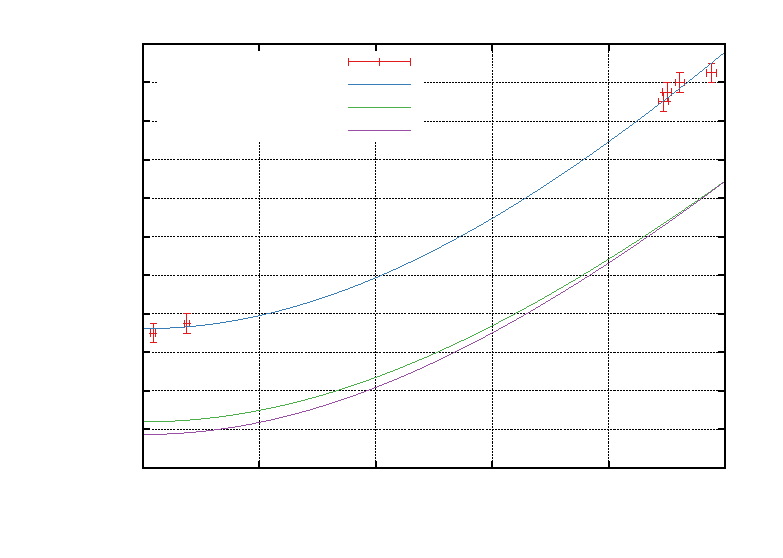
\includegraphics{./plots/strahlradien/strahlradius_50cm}}%
    \gplfronttext
  \end{picture}%
\endgroup

	\caption{Anpassung des Strahlprofils an die Messdaten für die Resonatorlänge $L = \SI{500 +- 4}{\milli\metre}$}
	\label{fig:strahlradius_50}
\end{figure}
\FloatBarrier
\begin{table}[t]
	\centering
	\begin{tabular}{SSSS}
\toprule
{$z \, / \, \si{\milli\metre}$} & {$\Delta z \, / \, \si{\milli\metre}$} & {$d \, / \, \si{\milli\metre}$} & {$\Delta d \, / \, \si{\milli\metre}$} \\
\midrule
12  & 2 & 0.74 & 0.01 \\
27  & 2 & 0.75 & 0.01 \\
32  & 2 & 0.76 & 0.01 \\
450 & 4 & 1.06 & 0.01 \\
483 & 4 & 1.10 & 0.01 \\
505 & 4 & 1.13 & 0.01 \\
554 & 4 & 1.18 & 0.01 \\
591 & 4 & 1.21 & 0.01 \\
618 & 4 & 1.23 & 0.01 \\
649 & 4 & 1.26 & 0.01 \\
666 & 4 & 1.28 & 0.01 \\
\bottomrule
\end{tabular}
	\caption{Messdaten zum Strahlprofil im Resonator der Länge $L = \SI{690 +- 4}{\milli\metre}$}
	\label{tab:strahlradius_70}
\end{table}
\begin{figure}[b]
	\centering
	% GNUPLOT: LaTeX picture with Postscript
\begingroup
  \makeatletter
  \providecommand\color[2][]{%
    \GenericError{(gnuplot) \space\space\space\@spaces}{%
      Package color not loaded in conjunction with
      terminal option `colourtext'%
    }{See the gnuplot documentation for explanation.%
    }{Either use 'blacktext' in gnuplot or load the package
      color.sty in LaTeX.}%
    \renewcommand\color[2][]{}%
  }%
  \providecommand\includegraphics[2][]{%
    \GenericError{(gnuplot) \space\space\space\@spaces}{%
      Package graphicx or graphics not loaded%
    }{See the gnuplot documentation for explanation.%
    }{The gnuplot epslatex terminal needs graphicx.sty or graphics.sty.}%
    \renewcommand\includegraphics[2][]{}%
  }%
  \providecommand\rotatebox[2]{#2}%
  \@ifundefined{ifGPcolor}{%
    \newif\ifGPcolor
    \GPcolortrue
  }{}%
  \@ifundefined{ifGPblacktext}{%
    \newif\ifGPblacktext
    \GPblacktexttrue
  }{}%
  % define a \g@addto@macro without @ in the name:
  \let\gplgaddtomacro\g@addto@macro
  % define empty templates for all commands taking text:
  \gdef\gplbacktext{}%
  \gdef\gplfronttext{}%
  \makeatother
  \ifGPblacktext
    % no textcolor at all
    \def\colorrgb#1{}%
    \def\colorgray#1{}%
  \else
    % gray or color?
    \ifGPcolor
      \def\colorrgb#1{\color[rgb]{#1}}%
      \def\colorgray#1{\color[gray]{#1}}%
      \expandafter\def\csname LTw\endcsname{\color{white}}%
      \expandafter\def\csname LTb\endcsname{\color{black}}%
      \expandafter\def\csname LTa\endcsname{\color{black}}%
      \expandafter\def\csname LT0\endcsname{\color[rgb]{1,0,0}}%
      \expandafter\def\csname LT1\endcsname{\color[rgb]{0,1,0}}%
      \expandafter\def\csname LT2\endcsname{\color[rgb]{0,0,1}}%
      \expandafter\def\csname LT3\endcsname{\color[rgb]{1,0,1}}%
      \expandafter\def\csname LT4\endcsname{\color[rgb]{0,1,1}}%
      \expandafter\def\csname LT5\endcsname{\color[rgb]{1,1,0}}%
      \expandafter\def\csname LT6\endcsname{\color[rgb]{0,0,0}}%
      \expandafter\def\csname LT7\endcsname{\color[rgb]{1,0.3,0}}%
      \expandafter\def\csname LT8\endcsname{\color[rgb]{0.5,0.5,0.5}}%
    \else
      % gray
      \def\colorrgb#1{\color{black}}%
      \def\colorgray#1{\color[gray]{#1}}%
      \expandafter\def\csname LTw\endcsname{\color{white}}%
      \expandafter\def\csname LTb\endcsname{\color{black}}%
      \expandafter\def\csname LTa\endcsname{\color{black}}%
      \expandafter\def\csname LT0\endcsname{\color{black}}%
      \expandafter\def\csname LT1\endcsname{\color{black}}%
      \expandafter\def\csname LT2\endcsname{\color{black}}%
      \expandafter\def\csname LT3\endcsname{\color{black}}%
      \expandafter\def\csname LT4\endcsname{\color{black}}%
      \expandafter\def\csname LT5\endcsname{\color{black}}%
      \expandafter\def\csname LT6\endcsname{\color{black}}%
      \expandafter\def\csname LT7\endcsname{\color{black}}%
      \expandafter\def\csname LT8\endcsname{\color{black}}%
    \fi
  \fi
  \setlength{\unitlength}{0.0500bp}%
  \begin{picture}(7200.00,5040.00)%
    \gplgaddtomacro\gplbacktext{%
      \csname LTb\endcsname%
      \put(1078,704){\makebox(0,0)[r]{\strut{} 0,3}}%
      \csname LTb\endcsname%
      \put(1078,1213){\makebox(0,0)[r]{\strut{} 0,35}}%
      \csname LTb\endcsname%
      \put(1078,1722){\makebox(0,0)[r]{\strut{} 0,4}}%
      \csname LTb\endcsname%
      \put(1078,2231){\makebox(0,0)[r]{\strut{} 0,45}}%
      \csname LTb\endcsname%
      \put(1078,2739){\makebox(0,0)[r]{\strut{} 0,5}}%
      \csname LTb\endcsname%
      \put(1078,3248){\makebox(0,0)[r]{\strut{} 0,55}}%
      \csname LTb\endcsname%
      \put(1078,3757){\makebox(0,0)[r]{\strut{} 0,6}}%
      \csname LTb\endcsname%
      \put(1078,4266){\makebox(0,0)[r]{\strut{} 0,65}}%
      \csname LTb\endcsname%
      \put(1078,4775){\makebox(0,0)[r]{\strut{} 0,7}}%
      \csname LTb\endcsname%
      \put(1210,484){\makebox(0,0){\strut{} 0}}%
      \csname LTb\endcsname%
      \put(2009,484){\makebox(0,0){\strut{} 100}}%
      \csname LTb\endcsname%
      \put(2808,484){\makebox(0,0){\strut{} 200}}%
      \csname LTb\endcsname%
      \put(3607,484){\makebox(0,0){\strut{} 300}}%
      \csname LTb\endcsname%
      \put(4406,484){\makebox(0,0){\strut{} 400}}%
      \csname LTb\endcsname%
      \put(5205,484){\makebox(0,0){\strut{} 500}}%
      \csname LTb\endcsname%
      \put(6004,484){\makebox(0,0){\strut{} 600}}%
      \csname LTb\endcsname%
      \put(6803,484){\makebox(0,0){\strut{} 700}}%
      \put(176,2739){\rotatebox{-270}{\makebox(0,0){\strut{}Strahlradius $w \, / \, \si{\milli\metre}$}}}%
      \put(4006,154){\makebox(0,0){\strut{}Abstand von der Strahltaille $z \, / \, \si{\milli\metre}$}}%
      \put(4006,4665){\makebox(0,0){\strut{}}}%
    }%
    \gplgaddtomacro\gplfronttext{%
      \csname LTb\endcsname%
      \put(3058,4602){\makebox(0,0)[r]{\strut{}Messwerte}}%
      \csname LTb\endcsname%
      \put(3058,4382){\makebox(0,0)[r]{\strut{}$\alpha \cdot w_\mathrm{exp.}(z)$}}%
      \csname LTb\endcsname%
      \put(3058,4162){\makebox(0,0)[r]{\strut{}$w_\mathrm{exp.}(z)$}}%
      \csname LTb\endcsname%
      \put(3058,3942){\makebox(0,0)[r]{\strut{}$w_\mathrm{theo.}(z)$}}%
    }%
    \gplbacktext
    \put(0,0){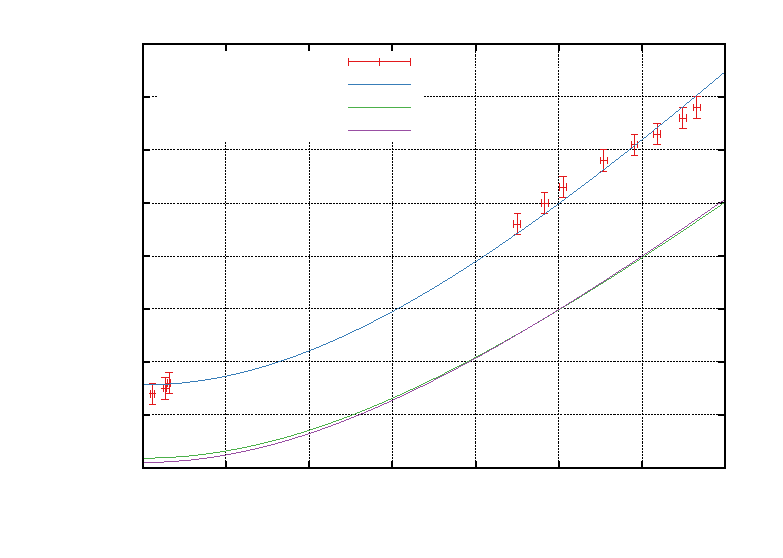
\includegraphics{./plots/strahlradien/strahlradius_70cm}}%
    \gplfronttext
  \end{picture}%
\endgroup

	\caption{Anpassung des Strahlprofils an die Messdaten für die Resonatorlänge $L = \SI{690 +- 4}{\milli\metre}$}
	\label{fig:strahlradius_70}
\end{figure}
\FloatBarrier
\begin{table}[t]
	\centering
	\begin{tabular}{SSSS}
\toprule
{$z \, / \, \si{\milli\metre}$} & {$\Delta z \, / \, \si{\milli\metre}$} & {$d \, / \, \si{\milli\metre}$} & {$\Delta d \, / \, \si{\milli\metre}$} \\
\midrule
10  & 2 & 0.67 & 0.01 \\
27  & 2 & 0.68 & 0.01 \\
442 & 4 & 1.04 & 0.01 \\
492 & 4 & 1.10 & 0.01 \\
542 & 4 & 1.16 & 0.01 \\
581 & 4 & 1.21 & 0.01 \\
639 & 4 & 1.26 & 0.01 \\
674 & 4 & 1.31 & 0.01 \\
708 & 4 & 1.36 & 0.01 \\
744 & 4 & 1.38 & 0.01 \\
\bottomrule
\end{tabular}
	\caption{Messdaten zum Strahlprofil im Resonator der Länge $L = \SI{795 +- 4}{\milli\metre}$}
	\label{tab:strahlradius_80}
\end{table}
\begin{figure}[b]
	\centering
	% GNUPLOT: LaTeX picture with Postscript
\begingroup
  \makeatletter
  \providecommand\color[2][]{%
    \GenericError{(gnuplot) \space\space\space\@spaces}{%
      Package color not loaded in conjunction with
      terminal option `colourtext'%
    }{See the gnuplot documentation for explanation.%
    }{Either use 'blacktext' in gnuplot or load the package
      color.sty in LaTeX.}%
    \renewcommand\color[2][]{}%
  }%
  \providecommand\includegraphics[2][]{%
    \GenericError{(gnuplot) \space\space\space\@spaces}{%
      Package graphicx or graphics not loaded%
    }{See the gnuplot documentation for explanation.%
    }{The gnuplot epslatex terminal needs graphicx.sty or graphics.sty.}%
    \renewcommand\includegraphics[2][]{}%
  }%
  \providecommand\rotatebox[2]{#2}%
  \@ifundefined{ifGPcolor}{%
    \newif\ifGPcolor
    \GPcolortrue
  }{}%
  \@ifundefined{ifGPblacktext}{%
    \newif\ifGPblacktext
    \GPblacktexttrue
  }{}%
  % define a \g@addto@macro without @ in the name:
  \let\gplgaddtomacro\g@addto@macro
  % define empty templates for all commands taking text:
  \gdef\gplbacktext{}%
  \gdef\gplfronttext{}%
  \makeatother
  \ifGPblacktext
    % no textcolor at all
    \def\colorrgb#1{}%
    \def\colorgray#1{}%
  \else
    % gray or color?
    \ifGPcolor
      \def\colorrgb#1{\color[rgb]{#1}}%
      \def\colorgray#1{\color[gray]{#1}}%
      \expandafter\def\csname LTw\endcsname{\color{white}}%
      \expandafter\def\csname LTb\endcsname{\color{black}}%
      \expandafter\def\csname LTa\endcsname{\color{black}}%
      \expandafter\def\csname LT0\endcsname{\color[rgb]{1,0,0}}%
      \expandafter\def\csname LT1\endcsname{\color[rgb]{0,1,0}}%
      \expandafter\def\csname LT2\endcsname{\color[rgb]{0,0,1}}%
      \expandafter\def\csname LT3\endcsname{\color[rgb]{1,0,1}}%
      \expandafter\def\csname LT4\endcsname{\color[rgb]{0,1,1}}%
      \expandafter\def\csname LT5\endcsname{\color[rgb]{1,1,0}}%
      \expandafter\def\csname LT6\endcsname{\color[rgb]{0,0,0}}%
      \expandafter\def\csname LT7\endcsname{\color[rgb]{1,0.3,0}}%
      \expandafter\def\csname LT8\endcsname{\color[rgb]{0.5,0.5,0.5}}%
    \else
      % gray
      \def\colorrgb#1{\color{black}}%
      \def\colorgray#1{\color[gray]{#1}}%
      \expandafter\def\csname LTw\endcsname{\color{white}}%
      \expandafter\def\csname LTb\endcsname{\color{black}}%
      \expandafter\def\csname LTa\endcsname{\color{black}}%
      \expandafter\def\csname LT0\endcsname{\color{black}}%
      \expandafter\def\csname LT1\endcsname{\color{black}}%
      \expandafter\def\csname LT2\endcsname{\color{black}}%
      \expandafter\def\csname LT3\endcsname{\color{black}}%
      \expandafter\def\csname LT4\endcsname{\color{black}}%
      \expandafter\def\csname LT5\endcsname{\color{black}}%
      \expandafter\def\csname LT6\endcsname{\color{black}}%
      \expandafter\def\csname LT7\endcsname{\color{black}}%
      \expandafter\def\csname LT8\endcsname{\color{black}}%
    \fi
  \fi
  \setlength{\unitlength}{0.0500bp}%
  \begin{picture}(7200.00,5040.00)%
    \gplgaddtomacro\gplbacktext{%
      \csname LTb\endcsname%
      \put(1078,704){\makebox(0,0)[r]{\strut{} 0,25}}%
      \csname LTb\endcsname%
      \put(1078,1074){\makebox(0,0)[r]{\strut{} 0,3}}%
      \csname LTb\endcsname%
      \put(1078,1444){\makebox(0,0)[r]{\strut{} 0,35}}%
      \csname LTb\endcsname%
      \put(1078,1814){\makebox(0,0)[r]{\strut{} 0,4}}%
      \csname LTb\endcsname%
      \put(1078,2184){\makebox(0,0)[r]{\strut{} 0,45}}%
      \csname LTb\endcsname%
      \put(1078,2554){\makebox(0,0)[r]{\strut{} 0,5}}%
      \csname LTb\endcsname%
      \put(1078,2925){\makebox(0,0)[r]{\strut{} 0,55}}%
      \csname LTb\endcsname%
      \put(1078,3295){\makebox(0,0)[r]{\strut{} 0,6}}%
      \csname LTb\endcsname%
      \put(1078,3665){\makebox(0,0)[r]{\strut{} 0,65}}%
      \csname LTb\endcsname%
      \put(1078,4035){\makebox(0,0)[r]{\strut{} 0,7}}%
      \csname LTb\endcsname%
      \put(1078,4405){\makebox(0,0)[r]{\strut{} 0,75}}%
      \csname LTb\endcsname%
      \put(1078,4775){\makebox(0,0)[r]{\strut{} 0,8}}%
      \csname LTb\endcsname%
      \put(1210,484){\makebox(0,0){\strut{} 0}}%
      \csname LTb\endcsname%
      \put(1909,484){\makebox(0,0){\strut{} 100}}%
      \csname LTb\endcsname%
      \put(2608,484){\makebox(0,0){\strut{} 200}}%
      \csname LTb\endcsname%
      \put(3307,484){\makebox(0,0){\strut{} 300}}%
      \csname LTb\endcsname%
      \put(4007,484){\makebox(0,0){\strut{} 400}}%
      \csname LTb\endcsname%
      \put(4706,484){\makebox(0,0){\strut{} 500}}%
      \csname LTb\endcsname%
      \put(5405,484){\makebox(0,0){\strut{} 600}}%
      \csname LTb\endcsname%
      \put(6104,484){\makebox(0,0){\strut{} 700}}%
      \csname LTb\endcsname%
      \put(6803,484){\makebox(0,0){\strut{} 800}}%
      \put(176,2739){\rotatebox{-270}{\makebox(0,0){\strut{}Strahlradius $w \, / \, \si{\milli\metre}$}}}%
      \put(4006,154){\makebox(0,0){\strut{}Abstand von der Strahltaille $z \, / \, \si{\milli\metre}$}}%
      \put(4006,4665){\makebox(0,0){\strut{}}}%
    }%
    \gplgaddtomacro\gplfronttext{%
      \csname LTb\endcsname%
      \put(3058,4602){\makebox(0,0)[r]{\strut{}Messwerte}}%
      \csname LTb\endcsname%
      \put(3058,4382){\makebox(0,0)[r]{\strut{}$\alpha \cdot w_\mathrm{exp.}(z)$}}%
      \csname LTb\endcsname%
      \put(3058,4162){\makebox(0,0)[r]{\strut{}$w_\mathrm{exp.}(z)$}}%
      \csname LTb\endcsname%
      \put(3058,3942){\makebox(0,0)[r]{\strut{}$w_\mathrm{theo.}(z)$}}%
    }%
    \gplbacktext
    \put(0,0){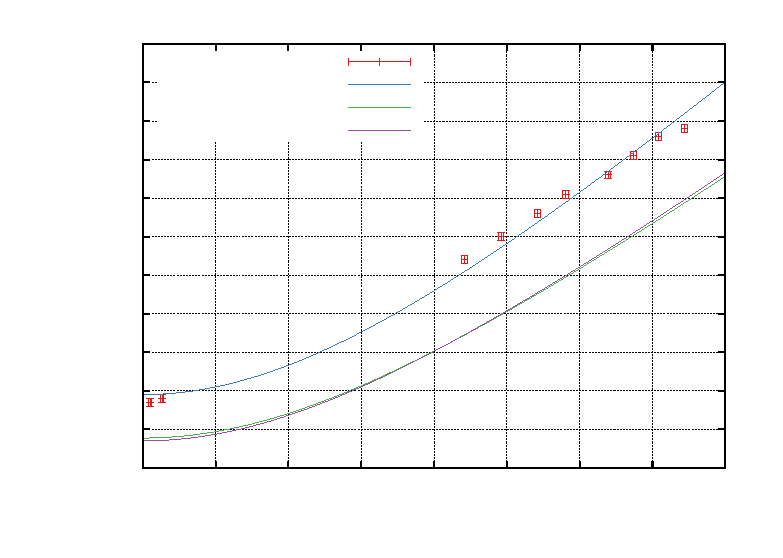
\includegraphics{./plots/strahlradien/strahlradius_80cm}}%
    \gplfronttext
  \end{picture}%
\endgroup

	\caption{Anpassung des Strahlprofils an die Messdaten für die Resonatorlänge $L = \SI{795 +- 4}{\milli\metre}$}
	\label{fig:strahlradius_80}
\end{figure}
\FloatBarrier
\begin{table}[t]
	\centering
	\begin{tabular}{SSSS}
\toprule
{$z \, / \, \si{\milli\metre}$} & {$\Delta z \, / \, \si{\milli\metre}$} & {$d \, / \, \si{\milli\metre}$} & {$\Delta d \, / \, \si{\milli\metre}$} \\
\midrule
7   & 2 & 0.59 & 0.01 \\
12  & 2 & 0.60 & 0.01 \\
35  & 2 & 0.63 & 0.01 \\
454 & 4 & 1.09 & 0.01 \\
474 & 4 & 1.13 & 0.01 \\
497 & 4 & 1.16 & 0.01 \\
543 & 4 & 1.21 & 0.01 \\
581 & 4 & 1.26 & 0.01 \\
628 & 4 & 1.34 & 0.01 \\
669 & 4 & 1.40 & 0.01 \\
768 & 4 & 1.54 & 0.01 \\
\bottomrule
\end{tabular}
	\caption{Messdaten zum Strahlprofil im Resonator der Länge $L = \SI{892 +- 4}{\milli\metre}$}
	\label{tab:strahlradius_90}
\end{table}
\begin{figure}[b]
	\centering
	% GNUPLOT: LaTeX picture with Postscript
\begingroup
  \makeatletter
  \providecommand\color[2][]{%
    \GenericError{(gnuplot) \space\space\space\@spaces}{%
      Package color not loaded in conjunction with
      terminal option `colourtext'%
    }{See the gnuplot documentation for explanation.%
    }{Either use 'blacktext' in gnuplot or load the package
      color.sty in LaTeX.}%
    \renewcommand\color[2][]{}%
  }%
  \providecommand\includegraphics[2][]{%
    \GenericError{(gnuplot) \space\space\space\@spaces}{%
      Package graphicx or graphics not loaded%
    }{See the gnuplot documentation for explanation.%
    }{The gnuplot epslatex terminal needs graphicx.sty or graphics.sty.}%
    \renewcommand\includegraphics[2][]{}%
  }%
  \providecommand\rotatebox[2]{#2}%
  \@ifundefined{ifGPcolor}{%
    \newif\ifGPcolor
    \GPcolortrue
  }{}%
  \@ifundefined{ifGPblacktext}{%
    \newif\ifGPblacktext
    \GPblacktexttrue
  }{}%
  % define a \g@addto@macro without @ in the name:
  \let\gplgaddtomacro\g@addto@macro
  % define empty templates for all commands taking text:
  \gdef\gplbacktext{}%
  \gdef\gplfronttext{}%
  \makeatother
  \ifGPblacktext
    % no textcolor at all
    \def\colorrgb#1{}%
    \def\colorgray#1{}%
  \else
    % gray or color?
    \ifGPcolor
      \def\colorrgb#1{\color[rgb]{#1}}%
      \def\colorgray#1{\color[gray]{#1}}%
      \expandafter\def\csname LTw\endcsname{\color{white}}%
      \expandafter\def\csname LTb\endcsname{\color{black}}%
      \expandafter\def\csname LTa\endcsname{\color{black}}%
      \expandafter\def\csname LT0\endcsname{\color[rgb]{1,0,0}}%
      \expandafter\def\csname LT1\endcsname{\color[rgb]{0,1,0}}%
      \expandafter\def\csname LT2\endcsname{\color[rgb]{0,0,1}}%
      \expandafter\def\csname LT3\endcsname{\color[rgb]{1,0,1}}%
      \expandafter\def\csname LT4\endcsname{\color[rgb]{0,1,1}}%
      \expandafter\def\csname LT5\endcsname{\color[rgb]{1,1,0}}%
      \expandafter\def\csname LT6\endcsname{\color[rgb]{0,0,0}}%
      \expandafter\def\csname LT7\endcsname{\color[rgb]{1,0.3,0}}%
      \expandafter\def\csname LT8\endcsname{\color[rgb]{0.5,0.5,0.5}}%
    \else
      % gray
      \def\colorrgb#1{\color{black}}%
      \def\colorgray#1{\color[gray]{#1}}%
      \expandafter\def\csname LTw\endcsname{\color{white}}%
      \expandafter\def\csname LTb\endcsname{\color{black}}%
      \expandafter\def\csname LTa\endcsname{\color{black}}%
      \expandafter\def\csname LT0\endcsname{\color{black}}%
      \expandafter\def\csname LT1\endcsname{\color{black}}%
      \expandafter\def\csname LT2\endcsname{\color{black}}%
      \expandafter\def\csname LT3\endcsname{\color{black}}%
      \expandafter\def\csname LT4\endcsname{\color{black}}%
      \expandafter\def\csname LT5\endcsname{\color{black}}%
      \expandafter\def\csname LT6\endcsname{\color{black}}%
      \expandafter\def\csname LT7\endcsname{\color{black}}%
      \expandafter\def\csname LT8\endcsname{\color{black}}%
    \fi
  \fi
  \setlength{\unitlength}{0.0500bp}%
  \begin{picture}(7200.00,5040.00)%
    \gplgaddtomacro\gplbacktext{%
      \csname LTb\endcsname%
      \put(946,704){\makebox(0,0)[r]{\strut{} 0,2}}%
      \csname LTb\endcsname%
      \put(946,1213){\makebox(0,0)[r]{\strut{} 0,3}}%
      \csname LTb\endcsname%
      \put(946,1722){\makebox(0,0)[r]{\strut{} 0,4}}%
      \csname LTb\endcsname%
      \put(946,2231){\makebox(0,0)[r]{\strut{} 0,5}}%
      \csname LTb\endcsname%
      \put(946,2740){\makebox(0,0)[r]{\strut{} 0,6}}%
      \csname LTb\endcsname%
      \put(946,3248){\makebox(0,0)[r]{\strut{} 0,7}}%
      \csname LTb\endcsname%
      \put(946,3757){\makebox(0,0)[r]{\strut{} 0,8}}%
      \csname LTb\endcsname%
      \put(946,4266){\makebox(0,0)[r]{\strut{} 0,9}}%
      \csname LTb\endcsname%
      \put(946,4775){\makebox(0,0)[r]{\strut{} 1}}%
      \csname LTb\endcsname%
      \put(1078,484){\makebox(0,0){\strut{} 0}}%
      \csname LTb\endcsname%
      \put(1714,484){\makebox(0,0){\strut{} 100}}%
      \csname LTb\endcsname%
      \put(2350,484){\makebox(0,0){\strut{} 200}}%
      \csname LTb\endcsname%
      \put(2986,484){\makebox(0,0){\strut{} 300}}%
      \csname LTb\endcsname%
      \put(3622,484){\makebox(0,0){\strut{} 400}}%
      \csname LTb\endcsname%
      \put(4259,484){\makebox(0,0){\strut{} 500}}%
      \csname LTb\endcsname%
      \put(4895,484){\makebox(0,0){\strut{} 600}}%
      \csname LTb\endcsname%
      \put(5531,484){\makebox(0,0){\strut{} 700}}%
      \csname LTb\endcsname%
      \put(6167,484){\makebox(0,0){\strut{} 800}}%
      \csname LTb\endcsname%
      \put(6803,484){\makebox(0,0){\strut{} 900}}%
      \put(176,2739){\rotatebox{-270}{\makebox(0,0){\strut{}Strahlradius $w \, / \, \si{\milli\metre}$}}}%
      \put(3940,154){\makebox(0,0){\strut{}Abstand von der Strahltaille $z \, / \, \si{\milli\metre}$}}%
      \put(3940,4665){\makebox(0,0){\strut{}}}%
    }%
    \gplgaddtomacro\gplfronttext{%
      \csname LTb\endcsname%
      \put(2926,4602){\makebox(0,0)[r]{\strut{}Messwerte}}%
      \csname LTb\endcsname%
      \put(2926,4382){\makebox(0,0)[r]{\strut{}$\alpha \cdot w_\mathrm{exp.}(z)$}}%
      \csname LTb\endcsname%
      \put(2926,4162){\makebox(0,0)[r]{\strut{}$w_\mathrm{exp.}(z)$}}%
      \csname LTb\endcsname%
      \put(2926,3942){\makebox(0,0)[r]{\strut{}$w_\mathrm{theo.}(z)$}}%
    }%
    \gplbacktext
    \put(0,0){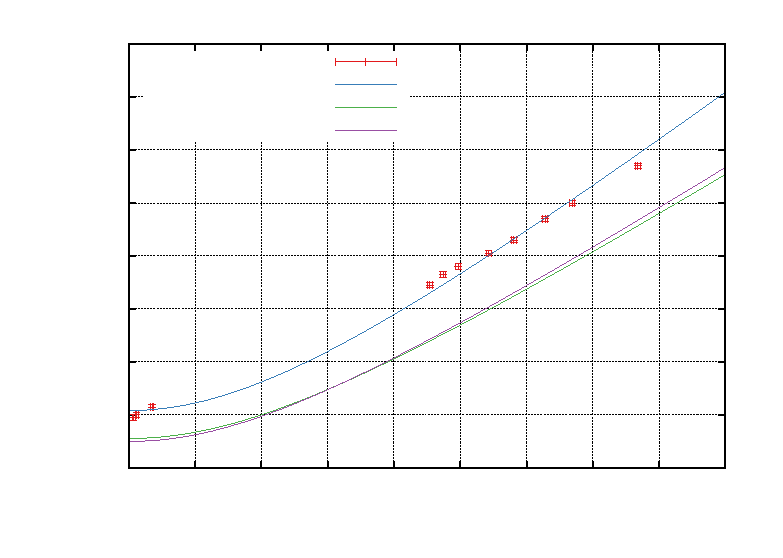
\includegraphics{./plots/strahlradien/strahlradius_90cm}}%
    \gplfronttext
  \end{picture}%
\endgroup

	\caption{Anpassung des Strahlprofils an die Messdaten für die Resonatorlänge $L = \SI{892 +- 4}{\milli\metre}$}
	\label{fig:strahlradius_90}
\end{figure}
\FloatBarrier


\end{appendix}

\end{document}
